\documentclass[10pt]{scrreprt}
\usepackage[utf8]{inputenc}
\usepackage{amsmath}
\usepackage{amsfonts}
\usepackage{amssymb}
\usepackage{graphicx}
\usepackage{listings}
\usepackage{usecases}
\usepackage{lmodern}
\author{Kim Rostgaard Christensen}
\title{Requirements as tests}
\subtitle{Automatic generation of test from structured requirements}
%%%%********************************************************************
\usepackage{microtype}
%\usepackage{times}
\usepackage[utf8]{inputenc}     
\usepackage[english]{babel}
\usepackage{color}
\usepackage{xcolor}
\usepackage{lipsum}
\usepackage{hyperref}
%%%%********************************************************************
% fancy quotes
\definecolor{quotemark}{gray}{0.7}
\makeatletter
\def\fquote{%
    \@ifnextchar[{\fquote@i}{\fquote@i[]}%]
           }%
\def\fquote@i[#1]{%
    \def\tempa{#1}%
    \@ifnextchar[{\fquote@ii}{\fquote@ii[]}%]
                 }%
\def\fquote@ii[#1]{%
    \def\tempb{#1}%
    \@ifnextchar[{\fquote@iii}{\fquote@iii[]}%]
                      }%
\def\fquote@iii[#1]{%
    \def\tempc{#1}%
    \vspace{1em}%
    \noindent%
    \begin{list}{}{%
         \setlength{\leftmargin}{0.1\textwidth}%
         \setlength{\rightmargin}{0.1\textwidth}%
                  }%
         \item[]%
         \begin{picture}(0,0)%
         \put(-15,-5){\makebox(0,0){\scalebox{3}{\textcolor{quotemark}{``}}}}%
         \end{picture}%
         \begingroup\itshape}%
 %%%%********************************************************************
 \def\endfquote{%
 \endgroup\par%
 \makebox[0pt][l]{%
 \hspace{0.8\textwidth}%
 \begin{picture}(0,0)(0,0)%
 \put(15,15){\makebox(0,0){%
 \scalebox{3}{\color{quotemark}''}}}%
 \end{picture}}%
 \ifx\tempa\empty%
 \else%
    \ifx\tempc\empty%
       \hfill\rule{100pt}{0.5pt}\\\mbox{}\hfill\tempa,\ \emph{\tempb}%
   \else%
       \hfill\rule{100pt}{0.5pt}\\\mbox{}\hfill\tempa,\ \emph{\tempb},\ \tempc%
   \fi\fi\par%
   \vspace{0.5em}%
 \end{list}%
 }%
 \makeatother
 %%%%********************************************************************

\definecolor{mygreen}{rgb}{0,0.6,0}
\definecolor{mygray}{rgb}{0.4,0.4,0.4}
\definecolor{mymauve}{rgb}{0.58,0,0.82}

% Define colors used for listings
\definecolor{dkgreen}{rgb}{0,0.6,0}
\definecolor{dkred}{rgb}{0.6,0,0}
\definecolor{gray}{rgb}{0.5,0.5,0.5}
\definecolor{mauve}{rgb}{0.58,0,0.82}
% Configuration for listings
\lstset{%
numbers=left,
frame=single,
numbers=left,
numberstyle=\tiny,
numbersep=15pt,tabsize=4,
flexiblecolumns=true,
keywordstyle=\color{blue},
commentstyle=\color{dkgreen},
basicstyle=\footnotesize\ttfamily,
stringstyle=\color{mauve},
numberstyle=\tiny\color{gray},
language=Java,
breaklines=true,
breakatwhitespace=true,
morekeywords={*,num,String,var,library,get,set} ,
}

\lstdefinestyle{usecase}{
  emptylines=1,
  breaklines=true,
  basicstyle=\ttfamily\color{black},
  escapeinside={@}{@},
  keywordstyle=\bfseries,
  morekeywords = {Scenario, Postconditions, Preconditions}
}
\usepackage{drawstack}

\newcommand{\imgdir}{./img/} % Set the folder which contains the specific images for the report

%TODO
% Write up 3-4 use cases. How they relate to each other. Maps to concept, and work on a conceptual level.

%TODO Using expected object state lifecycles (ordered list of states) to describe verification conditions.

%TODO section om mappings and levels of mappings. From Crude (having _one_ ast that is _the_ use case downto full semantics in language). One ast is what was done initially in Coverage_Tests.
%NOTE : A brief section on collection of asynchronous responses (expectations) that come in arbitrary order.

\begin{document}
\maketitle
 
\tableofcontents
\newpage

\begin{fquote}[ -- Johann Wolfgang von Goethe][The Sorrows of Young Werthe][1774]Misunderstandings and neglect occasion more mischief in the world than even malice and wickedness. At all events, the two latter are of less frequent occurrence.
\end{fquote}
\begin{abstract}
The world of software is has over the years been tainted with stories about failed projects. Almost everyone has his or her on story about a given software system, that did not solve the task, which it was designed to. This indicates; either a mismatch between requirements and solution, or simply erroneous requirement specifications. In the last decades more emphasis have been put on the agile methods, where smaller time-boxed iterations intricately contains every development phase; design, implementation, documentation and validation. Requirement refinement and elicitation may, however, be left dead-in-the-water and remain a \emph{de facto} waterfall phase with neither feed-back from implementation and validation, nor feed-forward to validation.
\end{abstract}

\chapter{Introduction}
\chapter{Introduction}
%TODO What is the scope of this? Is it for small/large projects? Long-lived projects? Continously evolving projects?
%How does this project want to change to actual problem.
%STATE THE ACTUAL PROBLEM - VERY SPECIFIC.
%State what is supposed to be done!
%TODO outline the three implementations, and say how they relate to each other.


Within the realm of software engineering, there exists a realm of requirement engineering there exists a domain of requirement elicitation and maintenance. In this realm, struggles of keeping documented requirements both consistent with -- and relevant to -- implementation often take place. A common procedure for gaining an upper hand in this struggle is to continuously, verify requirements though reviews and manual acceptance testing. This thesis proposes a tool and technique that is designed to alleviate some of the workload of continuous acceptance testing, and requirement change integration via code generation -- specifically test code generation. An idealized model of the process of this, is shown in figure \ref{fig:ideal_flow}. The concept is simple; construct requirements as use cases, map them to the implementation, generate tests from these requirements, and finally execute and validate these tests.
\begin{figure}[!htbp]
\centering
\includegraphics[width=0.7\textwidth]{\imgdir ideal_flow}
\caption{Ideal development flow}
\label{fig:ideal_flow}
\end{figure}
\section{Problem statement}
%TODO Overall problem. Provide a that enables tests to generated from structured use cases, without enforcing too many constraints on use case creation.
%The usability use cases are conditioned by their ease of use.
%TODO How to structure the use cases? Thiss is facilitated in the conceptual designs
Given the high rate of software project failures\cite{verner2008} \cite{charette2005}, and the general widespread requirement/implementation mismatch, we treat requirements and as incomplete and continuously evolving.
During the development life-cycle, additional domain knowledge is bound be acquired. This knowledge improves then general understanding of the problem domain, towards a better solutions. And often it also affects the requirements by making them more elaborate, complete, correct -- or event invalidate them. In any case, software development is an ongoing process, and use cases, and requirements must be, in a strict definition, expected to be incomplete, inaccurate and part of the development process.\bigskip

\noindent Integrating requirements deeper into the development can be -- and is -- done by adding a reference system from documentation to implementation files or components. This way, automated system can send out reminders to developers on which documents should be review, whenever a change has happened in a component.
Documentation, however, is usually written in natural language, with all the befits and ambiguities that follows.\bigskip

\noindent In this thesis, one of the goals is to add this feedback channel via generated acceptance tests. It is believed that if these tests are linked to the requirements, then implementation changes that affect requirements, will change the tests, which then will verify that the system still works as intended. But to be able to actually generate requirements from tests, we need to integrate some measures into the development process. A design of a development process is explained in the next section.\bigskip

\noindent Related challenges, faced by software engineers and developers, are requirement requirement documentation decay and inconsistency, and  by long-lived projects that continuously add features and components, is maintenance of requirements while adding new ones. This increases the risk of requirement documentation decay and inconsistency significantly. For example, a new requirement that allows users to access some information unauthenticated, may contradict a previous requirement.
Requirement maintenance is usually a time-consuming and tedious task with little -- immediately -- added value. When, for example, an implementation-specific constraint is forcing a requirement change, the change may propagate to the requirements, but not back into the validation.\medskip

\noindent When kept up-to-date and well-structured requirements usually map nicely to integration tests (either manual or automatic), but maintenance is needed for both if requirements change. It would therefore be very desirable to formalize requirements so that changes propagate to tests automatically.\medskip

\noindent If the requirements are formalized in a sufficiently structured way, and annotated with references to the implementation, we would be also able to automatically generate system tests from them. By generating these tests, we effectively provide a feedback channel from implementation to requirements, as these tests will serve as a link between requirements and implementation.\medskip

\noindent The tool that will be a product of this thesis, should support a technique that is able to extract the essential information, from informally specified -- yet structured -- information. Keeping as close to natural language as possible.

\section{Project}
This thesis proposes a tool designed for writing use cases coupled with an implementation mapping process. It is meant to provide a link between requirement and implementation through tests generated from structured implementation-mapped requirements. The generated tests will serve as a behavioral-validation mechanism meant for continuously be run against the implementation to assert that requirements are met throughout the evolution of the system under development.\medskip

\noindent The overall concept is illustrated in figure \ref{fig:tests-relation-to-implementation} that show requirements that are linked to artifacts from the implemented system, such as model classes in interfaces. The requirements will generate tests using the implementation artifacts links (mappings). Tests will run against the implementation and feed back reports that reveals whether the requirement behavior is working in the implementation or not.\medskip
\begin{figure}[!htbp]
\centering
\includegraphics[width=0.5\textwidth]{\imgdir tests-relation-to-implementation}
\caption{Concept of mapping from requirements to implementation}
\label{fig:tests-relation-to-implementation}
\end{figure}

\noindent Doing this will provide a general methodology for mapping requirements to implementation -- and vise versa -- that is \emph{feasible}. Feasible in the sense that is does not increase the number of extra man-hours spend on development significantly and scalable.\medskip

\noindent Some systems may be more testable than others, and the meaning of the design of the system is facilitated through a discussion of the case study system (section \ref{ssec:case-study-system-intro}).


\subsection{Overall concept}
In addition any activities already in place within the development of a software product (code writing, reviews, stakeholder meetings), a few more needs to be added for the different stakeholders to support use case test generation.\medskip

\noindent For every use case -- or change to an existing use case -- the system should generate a new set of tests, possibly replacing old tests. This process requires the participation of three different actors; the use case writer (Writer), the use case mapper (Mapper) and the system designed for generating and running tests (Testing system).\medskip

Figure \ref{fig:use_case_creation_activity_diagram} shows an activity diagram involving these actors. The Writer 
\begin{figure}[!htbp]
\includegraphics[width=0.95\linewidth]{\imgdir use_case_creation_activity_diagram}
\centering
\caption{Use case creation with different actors}
\label{fig:use_case_creation_activity_diagram}
\end{figure}
\noindent The basic idea is that sufficient structure in requirement formalization may enable tests to be generated directly from requirements fully automatically. To facilitate this, it means that requirements should be written with a strong focus on testability, and try to avoid non-realizable requirements. This, as a side effect, may increase the motivation for quantifying, constraining and refining requirements. As an example: \emph{Who} will perform this action, and how are the outcomes expected to be presented/received?\medskip

\noindent These questions should -- preferably -- be answered by the customer of the system, and mapped by a developer to actual functionality that may then be tested with regards to the behavior described in the requirements. So, in essence, the very basic use case; ``Administrator creates a new user'' with the postcondition ``The new user is created in the system'' should result in a test that, in some way, performs the ``add user'' action of the Administrator actor, and then verifies it against the postconditions. Ideally: With an appropriate level of detail provided in the use cases, and a grain of automated (and manual) mapping to domain concepts will enable automatic generation of acceptance tests. These can then be combined with a continuous integration service that runs the tests and reports results to developers.\medskip

\noindent The project will use the requirements from an existing system as a case study and build up a structure of these, so that test generation from them is possible. During this process, we will investigate how to structure requirements so that we can generate tests directly from them and map implementation to requirements. In doing this, we want to identify general patterns and constraints in the structure introduced to our requirements in the case study system to be able to apply them to other projects. In general, we will investigate to which extent this idea can be applied, and try to implement a translation tool that is able to translate a representation of a use cases into a tests case.\medskip

\noindent The project is considered to be derived from the test-driven development methodology (see section \ref{ssec:test-driven-development}). Lifting it from its typical application of integration testing onto the new level of acceptance testing. This process is meant to be tool-assisted, so that tests may be generated automatically, but the mappings to the system needs to be done by hand.\medskip

\noindent The tool we want to build here aims in usage to be integrated in an existing development procedure, with a low learning curve that enables a broad range of programmers to gain better integration of use cases into the development process.

\subsection{Case study system}
\label{ssec:case-study-system-intro}
This thesis uses the software project ``OpenReception'' as case study. The project aims to provide a drop-in replacement for an existing system, and therefore has relatively fixed requirements that are extracted from the workings of the existing system.The case study system is developed and released under an open source license and any implementation details are therefore public domain and not covered by any non-disclosure agreements.

\subsection{Outline}
The development of the case study system coined the idea of test generation from structured use cases, and spawned two implementations, than founded the basis of this project. The first was test generator, built as an auxiliary project, with no direct link to main project, other than the knowledge of which interfaces it exposed, and the serialized data structures it transmitted. It, thus, had a no direct implementation link, and every change in implementation had to propagated manually.\medskip
\begin{figure}[!htbp]
\centering
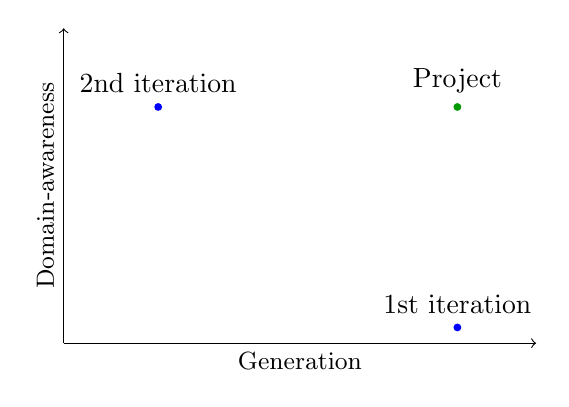
\begin{tikzpicture}

% horizontal axis
\draw[->] (0,0) -- (6,0) node[anchor=north,midway] {\small Generation};

% vertical axis
\draw[->] (0,0) -- (0,4) node[anchor=south,rotate=90,midway] {\small Domain-awareness};

\draw (5,0.2) node[circle,fill,inner sep=1pt, fill=blue, label=above:1st iteration] {};
\draw (1.2,3.0) node[circle,fill,inner sep=1pt, fill=blue, label=above:2nd iteration] {};

% Project dot
\draw (5,3) node[circle,fill,inner sep=1pt, fill=dkgreen, label=above:Project] {}; 

\end{tikzpicture}
\caption{Project parameters and key points}
\label{fig:project_parameter_plot}
\end{figure}
\noindent In the second iteration, the generated tests were later manually translated (programming language-wise) into a new set of tests that re-used the implemented code, and added what we defined as ``Domain-awareness''. This was done by, again manually, writing up a set of support tools that tried to mimic the domain model of the case study system. So, any actor or general domain concept would have an appropriate source code class in this tool set. It imported most of the interfaces and model classes from main code base of the case study system, so any implementation change would be propagated to -- or lead to compilation error in -- the test support tools. Having the domain-awareness helped linking requirements to tests, and -- indirectly -- implementation. But this implementation was not without its flaws.\medskip

\noindent Having written \emph{everything} manually in second iteration had two problems; the coverage was questionable -- did we cover all branches of the use cases? And, how should we propagate requirement changes to these tests? The idea of combining the test generation with domain-awareness would allow for a mapping between requirements in implementation that enable changes in either to be propagated to the other. Figure \ref{fig:project_parameter_plot} shows the parameters that we design after, and how the different implementations a located in this space. The figure will be repeated throughout the thesis to indicate where in this space the current section operate.

\section{Related work}
This section contains a brief overview of the related works, founded during the background research phase of this project.\medskip

\noindent John Rushby\cite{rushby2008automated} proposes that tests can be generated from requirements, \emph{if} these are already in an executable form, commonly found in model based software engineering. He identifies that there is a problem with loops in models as well. In the project from this thesis, the requirements are not executable, but merely text that is explicitly mapped to implementation.\medskip

\noindent Angelo Gargantini et al. proposes model checking techniques to generate tests from requirements\cite{gargantini1999using}. The scope of this, however, appears to be mostly on software cost reductions in the field of safety-critical software, and is too formal in nature to mainstream software development.\medskip

\noindent A, not strictly related, but very interesting concept that may support this project, is a textual analysis with the purpose of building up an initial conceptual (domain) model for use in the early development stages\cite{kop2010natural}. This would aid our project with a mapping suggestions, based on an analysis of what is written in the use cases.\medskip

\noindent In summary: There exist already methods and tools that support the formalization or structuring of requirements, but there seems to be a lack of motivation for applying them widely. The scope of them are either model-based software engineering, or safety-critical systems. The scope of this project is to provide an approach that is applicable in a wider array development environments -- without restrictions on software engineering paradigm, or target system market. It would however \emph{not} be suitable for safety-critical systems as it is very informal.

\section{Glossary}
In this section brief glossary from the problem domain is provided to cover the basic terminology used in the use cases.
\begin{description}
  \item[Customer:] The person in the role of purchasing the software. Assumed to have little or no knowledge about formalism, modeling or programming.
  \item[Contact:] A person or group known to the system -- i.e. previously created with contact details such as phone numbers and email addresses.
  \item[Receptionist:] A user in the system able to handle incoming calls by forwarding them or taking a message.
  \item[Caller:] Anyone who dials a phone number handled by the system. They are not known by the system \textit{a priory}, but the system \textit{may} store previously entered data that serves as a cache.
  \item[PBX:] Private Branch Exchange. A local phone switchboard with built-in logic that determines the flow and destination of a phone call based on dial-plans. Common PBX's capabilities phone queues, Interactive Voice Response (IVR) menus and transfers to either local extension, or external extension. A PBX can be either a special-purpose hardware device, or a software implementation running on regular general-purpose PC hardware. These are referred to as hard- and soft-PBX's, respectively.
  \item[Dial-plan:] A decision system that decides what to with a call from a set of rules, such as ``if the time of day is after 17 o' clock, send to voice mail'', or ``if the callee extension is +45 1234 5678'', put the call straight trough to manager's extension''. The concrete syntax is, of course closer to a programming language, and largely dependent on which PBX is used.
\end{description}
This glossary is incomplete, with regards to the domain model, but should be sufficient background for interpreting the following use cases.

\chapter{Top-down}
\subsection{Evolution of software engineering}
The natural evolution of software engineering points towards increasing the level of abstraction, moving closer to the usage models that they try capture. Another benefit of using models is that they communicate much better than, for instance, source code. Whereas source code is usually filled with non-essential implementation-specific details, models aim only to capture the essence of what it represents. Models, lacking these details, are challenging to execute. An doing so requires a great deal of extra work, filling out the details with either code snibblets or equivalent constraints -- such as OCL.\footnote{Object Constraint Language - part of UML}\\\\
One problem with this approach is a that much technical knowledge is required to formulate the models, OCL constraints and/or snibblets required for the system to function. For most technical staff it feels like meta-programming that keeps them from doing real programming.
\\\\
Ideally, the person requesting the software being modeled (the customer), should do a lot of the modeling by him/herself. This, however, has historically proven itself infeasible as customers rarely know much about modeling or programming, and if they did, would probably not be requesting software but rather making it on their own.

% Stub - I don't know where it should go;
\subsection{Bad requirements}
In software engineering there is a rule of thumb saying that requirements should be testable. This probably originates from the more general rule that goals should be measurable, recognizing that a requirement is ultimately a goal and a test is a actually a measure. Having this in mind can prevent a fair amount of bad requirements.
% Something about the level of detailm the completeness and feedback loop. Prototyping an agile development.
%\section{Terminology}
%\subsection{Three kinds of models}
%This document will use three descriptions for models, which cover;
%\subsubsection{Informal models}
%Informal models are used to describe models whose primary purpose is serve as a communication or documentation tool, not have strict semantics and cannot be used for code generation or model-checking.
%\subsubsection{Formal models}
%Formal models, which can be used for verification -- such as Z or VDM or plain math. Anything that has strict semantics and can be used to unambiguously generate code.
%\subsubsection{Meta-models}
%Meta-models that model other models, such as UML.

\section{Background}

%TODO more on this story. Something that leads to the discovery of a structure and pattern of use cases and tests. ALSO IMPORTANT; Add general section on tests (background and exisiting solutions) - and how this solution wishes to improve it.

\chapter{Background}
%TODO review this section and make it fit with next one.
This chapter provides the historical background and motivation for the idea that eventually became the topic of this thesis. It also gives a brief overview of the design and implementation of the case study system used in this thesis.

.. provides a brief introduction to software testing, test-driven development and how these relate to, and differ from this project.

\section{Software testing}

\subsection{Test-driven development}
A development methodology that emerged around the millennium, and have been looking very promising, is test-driven development. I focuses on -- as the name would also implicate -- tests before anything else. The basic work-flow is to first write tests, then refactor the code base of the system under development until the test passes. Then, to make sure the refactored code does not break existing functionality, all the previously written tests must be run. This work-flow is illustrated in the flow chart shown in \ref{fig:test-driven-development-flow}.

\begin{figure}[!htbp]
\centering
\includegraphics[scale=0.6]{\imgdir test-driven-development-flow}
\caption{Basic work-flow of test-driven development}
\label{fig:test-driven-development-flow}
\end{figure}Some of the arguments for using test-driven development is that it enables continuous regression testing. It focuses strongly on building the object and components that are needed rather than the ones that are thought to be needed. And it also lowers the gap between component design, and feedback.\cite{george2003}. By feedback is meant developer feedback -- whether the component works or not.\\
Test-driven development, in its nature, encourages code to be written testable. If a test is written prior to the code, then -- obviously -- the code written will be testable, or it will not pass the tests that originated it. This often means better code reuse and smaller, more loosely coupled components. This is probably due to the fact that when you write tests, it is often the case that you repeat some actions over and over again.\\\\
In this thesis, the methodology used is similar to the one found in test-driven development, in the way that you \emph{can} build tests from your use cases before the implementation. But unlike test-driven development it does dictate a specific point in development process where you should add the tests.\\
Instead it focuses on a tool-assisted generation of tests scopes to achieve a very broad coverage of requirements. So basically, it gives you the outline of what to test, and which domain concepts are needed for the test.

\subsection{Continuous integration}
Continuous integration is a methodology, that u

 that supplements

 to Test-driven development.


\section{Tests glossary}
In this section brief glossary from the test domain
\begin{description}
  \item[Test coverage:] The tests coverage is an indication of how many of the branches system is actually covered by the tests. So, a simple function with a single \emph{if-else} branch, that had a test that covered only the \emph{if} branch would have a coverage of 50\%. If there was also a test for the \emph{else} branch, the coverage would reach 100\%. Test coverage applies to every level of testing, from acceptance tests to unit tests.
  \item[White-box test:] A white-box test treats the system as a transparent box where all the internals are known. From these known internals, tests can be written to take a specific code path within the component under test. Unit tests are an example of a white-box test, as it tests the known internals of the unit. In the case study system, white-box tests are used to verify API's and system functionality -- effectively testing multiple API's in a single test.
  \item[Black-box test:] Treats the system as an unknown entity which responds to external stimuli. Nothing is known about the internals of the entity, and by by applying the stimuli, the entity will respond -- hopefully -- in the expected way. The Stimuli-organism-response (figure \ref{fig:sor-model}), which is used areas such as behavioral psychology, graphically depicts the concept very well.
  \item[Unit test:] Is a detailed test of a single unit in the system. While the size of the unit is not strictly defined, a unit is typically a single file or class in software systems. A unit test is a white-box test that focus on broad test coverage.
  \item[Integration test:] Is a test that treats a component, or set of components as a combined entity, and tests it as a black-box system. Integration testing is linked to functional requirements, but may also refer to non-functional requirements, such as behavior under load -- which is known is stress-testing.
  \item[Test harness:] An artificial environment that surrounds a test, supplying it with the resources and API's it needs. An example of a resource could be a database layer that supplies the test with the objects it needs. The harness does not need to provide real objects, but is free to return mock objects to the test, rather than having to deal with actually connecting to a database.
  \item[Acceptance test:] Test system as it should work %  is a test conducted to determine if the requirements of a specification or contract are met. It
\end{description}
\begin{figure}[!htbp]
  \centering
  \includegraphics[scale=0.6]{\imgdir sor-model}
  \label{fig:sor-model}
  \caption{Stimuli-organism-response model. Used -- for instance -- in psychology, but is analogous black-box testing}
\end{figure}

\section{Case study system}
Back in the fall of 2011, a physicist, an electrical engineer a systems programmer, three entrepreneurs and a software engineering student founded a small business. I was created to solve one grave problem that the entrepreneurs had; their current software system was becoming a larger and larger annoyance to them due to lack of upgrades and existing bugs that was never going to be fixed. The latter was due to the fact that the company supporting it, went bankrupt. Thus, a plan was laid to re-engineer a system that would serve as a drop-in replacement for their current one -- only this time as an open source system, so that at least there was a possibility to hand over support contracts to other suppliers, avoided their previous vendor lock-in.\\\\
The three entrepreneurs were in the business of ``reception hosting''. About one year after, the first conceptual prototype emerged, and by the end of 2013, an alpha version of the product was ready to be tested and hardened for production use. However, due to the high level of asynchronism, and low level of explicit coordination -- which was by design -- regressions became an increasing problem. And when the requirements also started to change, a dire need for automated, and usage-oriented testing became evident.


\subsection{Problem domain glossary}
In this section brief glossary from the problem domain is provided to cover the basic terminology used in the use cases.
\begin{description}
  \item[Customer:] The person in the role of purchasing the software. Assumed to have little or no knowledge about formalism, modeling or programming.
  \item[Contact:] A person or group known to the system -- i.e. previously created with contact details such as phone numbers and email addresses.
  \item[Receptionist:] A user in the system able to handle incoming calls by forwarding them or taking a message.
  \item[Caller:] Anyone who dials a phone number handled by the system. They are not known by the system \textit{a priory}, but the system \textit{may} store previously entered data that serves as a cache.
  \item[PBX:] Private Branch Exchange. A local phone switchboard with built-in logic that determines the flow and destination of a phone call based on dial-plans. Common PBX's capabilities phone queues, Interactive Voice Response (IVR) menus and transfers to either local extension, or external extension. A PBX can be either a special-purpose hardware device, or a software implementation running on regular general-purpose PC hardware. These are referred to as hard- and soft-PBX's, respectively.
  \item[Dial-plan:] A decision system that decides what to with a call from a set of rules, such as ``if the time of day is after 17 o' clock, send to voice mail'', or ``if the callee extension is +45 1234 5678'', put the call straight trough to manager's extension''. The concrete syntax is, of course closer to a programming language, and largely dependent on which PBX is used.
% \item[Domain concept] are usually also present in the mapping, and are usually mapped directly to a class.
%Use case definition: An event that describes behaviors and it's written from a user's perspective.

\end{description}
This glossary is incomplete, with regards to the domain model, but should be sufficient background for interpreting the following use cases.\\\\

\section{Business model and existing system}
The customer -- the Danish business Responsum -- sells what is called a hosted reception service. Their primary customer segment are other businesses -- both large and small. They employ a number of receptionists that answer phone calls on behalf of these businesses. They perform receptionist tasks as though they were physically located on the premises of those businesses, and have access to a lot of employee data, such as employee information, phone numbers and calendars. This information is continuously maintained by a number of service agents, usually by transferring data between systems manually.\\\\
Throughout the last ten years, they have used a COTS\footnote{Commercial Off The Shelf} system for this task, that is now showing its age. The system handles phone call routing, call handling (playing greetings and Interactive Voice Response (IVR) menus), presents reception information, manages call routing plans and reception information.
\begin{figure}[!hbpt]
\centering
\includegraphics[width=0.8\textwidth]{\imgdir frontdesk-client-ui}
\caption{Screenshot of the receptionist frontend of the existing system}
\label{fig:frontdesk_screenshot}
\end{figure}
The system is proprietary and abandoned by the developers and is still affected by open bugs and issues. Furthermore, the customers of Responsum are expressing an increasing interest in integrating their own system with the Responsum's system. An example of an integration could be calendar synchronization to lower the manual workload of their service agents.

\section{Replacement system}
This section gives a short introduction to the system, its architecture and design and the development process that ultimately motivated the test approach, that is the topic of this thesis.\\\\
\begin{figure}[!hbpt]
\centering
\includegraphics[width=0.8\textwidth]{\imgdir openreception-client-ui}
\caption{Screenshot of the receptionist frontend of the replacement system}
\label{fig:openreception-client-ui}
\end{figure}OpenReception web-based software/telephony system. It is a system designed to enable receptionists to handle incoming calls, and provide then with the appropriate information so that they may divert or directly handle the calls. The system is designed with high availability in mind with many -- largely independent -- components that are loosely coupled. This limits the Domino-effect, where one faulty component can take down another for no other reason than the fact that they are partitioned together.\\ This component-oriented design has also helped the testing process, as it enabled individual components to be tested and verified independently of the others. A screenshot of the receptionist client of the replacement system can be seen in figure \ref{fig:openreception-client-ui}.

\section{Project scope}
The fundamental requirements for the system originates directly from the fact, that is is supposed to be a drop-in replacement of an existing system. It should therefore, as a bare minimum, mirror the features of the existing system.\\
However, the current system has been in production for over ten years and lessons-learned has taught the customer how the system should be improved. Another thing that had to be considered, was the fact that the current system had proven it's stability. Despite being far from perfect, it was certainly usable and provided the technical means for the customer to keep the gears of their business model oiled.

%TODO maybe add a list of requirements.
%TODO features broke all the time, when was the system done?, Jenkins was introduced ...
%Use cases are stored in a wiki.

\section{Chosen architecture}
Being that the existing system was considered stable, and critical infrastructure, the replacement system was designed with simplicity, and high fault resilience in mind. This means that we tried to provide fall-back mechanisms for most of the system rather than over-eagerly handle every potential fault. The component diagram in figure \ref{fig:component_diagram} shows the architecture, and also gives away some hints about which components are critical, and which are not. Basically, the most critical path is the one that originates from the ``Receptionist Client'' and ends in the ``SIP trunk'' component. These components are considered soft real-time components and are essential for an operation. Fallout of any of these components means direct financial loss for the customer. Fallout of any of the other components (except for SIP Phone, which is actually part of the critical path mentioned above) are tolerated in the design, and the stateless nature of REST (see section \ref{sec:rest}) enables us to maintain caches that can supply clients with the data they need for handling calls.

%Something about fault handling, and about not knowning the "failure space"
%TODO add explanation of the figure, the components and the interfaces.
\begin{figure}[ht]
\centering
\includegraphics[width=0.9\textwidth]{\imgdir component_diagram}
\caption{Component diagram}
\label{fig:component_diagram}
\end{figure}

\section{Implementation}
\todo[inline]{Add nice introduction here}
\subsection{Fault tolerance}
Fault tolerance is built into the system, by first decomposing the system into a lot of smaller parts, reduce the amount the amount of communication (in particular; two-way communication) needed for the system to function, at least partially.

\subsection{Stateless architecture}
\label{sec:rest}
We are, like many others contemporary developers, using REST \footnote{(\textbf{RE}presentational \textbf{S}tate \textbf{T}ransfer)}. It is a reasonably new, and non-standardized (by any comity) techonology for building Web-connected API's. It is a client/server protocol that bases itself upon some very simple principles that enables high scalabilty by it's stateless design, This stateless design enables API providers to partition and cache their resources better, as they do not need to synchronize across partitions.\\
Automated system testing is also simplified quite a bit, when you don't need to take into account a protocol state.

\subsection{Loose coupling of components} 
In order to minimize the damage of a component failing, we have further atomized the REST API's that we created into smaller services, each responsible for only handling one single task. This is what is, informally, defined as the ``bulkhead pattern''. Originating from naval vessel floating compartments, that was composed of several individual bulkheads. These bulkheads could then be closed off, in case of a leakage in one of them. A parallel to software engineering is to divide your application into separate operating system processes that can be terminated if they start to leak memory, consume excessive amounts of CPU time, or merely lock up. Sometimes, killing worker processes is used as a preemptive method of assuring that processes are kept under control. The Apache HTTPD web server uses this strategy by maximizing the number of requests\footnote{http://httpd.apache.org/docs/2.2/mod/worker.html} a worker process may serve before being terminated and replaced.\\
In our architecture, we have divided the database operations, dialplan generation, CDR\footnote{Call Detail Records: records of call duration and other information used for invoicing} into dedicated servers, that may be replaced -- even while in production.

\subsection{Reactive application}
\label{ssec:server_notifications}
As an extension of the the stateless client/server architecture, a server notification-push pattern has also been added. This enables us make the user interface reactively update to global state changes, rather than having to poll for these changes periodically. It was the optimal way we could get the client interface to respond to system events in real-time. It ultimately also became an important component in testing, as we could use it as a mean to validate causal relationship of actions and events (for instance; a hangup action on a phone would lead to a hangup event notification).\todo{. maybe add a reference to the causality section}

\section{Testing strategy}
\label{sec:background-testing-strategy}
%NOTE This one is moved from first-iterations chapter.
As development progressed, it became increasingly difficult and time consuming to verify the correctness of the implementation by manually running the acceptance tests, which basically involved; performing an incoming call via a phone, picking up the call via the system, accept the call on another phone and then perform the actual use case scenario. This could, for example, be to forward the call and signal an idle state to system. Other issues with this manual approach was that is was time-consuming and was easy to perform in an incorrect order, thus leading to false negatives in test runs. Clearly the project could benefit from investing time in scripting the setup and tearing down of the state which was need to perform the manual tests.
During the progression of the project, it became more and more clear to us that we were constrained by two parameters, in regards to testing:
\begin{itemize}
  \item We needed to verify the the functionality of system as a whole, and argue that it was free of instabilities. This functionality was defined in the use cases.
  \item We had very limited man-hours available and, thus, had to prioritize very aggressively on what level to tests on.
\end{itemize}
\begin{figure}[ht]
\centering
\includegraphics[width=0.6\textwidth]{\imgdir receptionist_workflow}
\caption{Labeled activity diagram of the basic workflow of a receptionist}
\label{fig:receptionist_workflow}
\end{figure}
Being that the system consisted of a number of loosely coupled components, some of them not under our control, we decided to focus on writing up black-box tests focusing on verifying the behavior of the individual components, or multiple connected components.
Furthermore, we wanted to automate this using a continuous integration service that could run our tests for us, and provide us with reports on regressions, or identified bugs. But first, a proper level of testing had to be chosen.

\subsection{Level of testing}
\label{ssec:level-of-testing}
We chose path of assuming everything worked and, thus,  built tests from the perspective of how it should work. So we basically treated the system as a block-box system and abstract away as many implementation details as possible. For this purpose, we and built a ``robot-receptionist'' and a ``robot-caller''. These ``robots'' acted as clients and connected to the \textbf{REST-Data}, \textbf{REST-Call}, \textbf{REST-SIP} interfaces from figure \ref{fig:component_diagram}.\\\\

\subsection{Coverage of testing}
In order to test the system, using the black-box method, we needed to formulate the tests in a way that provided the broadest coverage possible. To achieve this, we crafted a set of activity diagrams from the use cases of the system (see figure \ref{fig:receptionist_workflow}). From this, we could assert that every ``happy path'' use case was covered, by covering every path of the activity diagram.

\subsection{Generation of tests}
To make sure that all paths were covered, every activity node got labeled. Any unique path through the activity diagram should then correspond to a use case, but more importantly; be realized by a test. To achieve this, we constructed a set of tools that, among other things contained the ``robots'' discussed briefly in section \ref{ssec:level-of-testing}.

\todo{.\\ This listing should probably be moved to a later chapter.}
\begin{lstlisting}[language=Python, caption=Example of a generated test, label=fig:python_test]

# Inherit Test_Case class from forward_call generalization.
from forward_call import Test_Case

class Sequence_Diagram (Test_Case):
  def test_Run (self):
    try:
      Incoming_Call_ID = self.Request_Customer_Call ()
      Outgoing_Call_ID = self.Receptionist_Places_Call 
                               (Number = self.Callee.extension)
      self.Callee_Receives_Call ()
      self.Receptionist_Hears_Dialtone ()
      self.Callee_Accepts_Call ()
      self.Receptionist_Hangs_Up (Call_ID = Outgoing_Call_ID)
      self.Callee_Receives_Hang_Up()
      self.Teardown ()
    except:
      self.Teardown () # Cleanup processes started
      raise            # Re-raise exception so that 
                       # test fails after we cleaned up
\end{lstlisting}

\todo[inline]{Mostly notes and stubs from hereon}.

\section{Testing}

\subsubsection{Acceptance testing}
%TODO: STUB, explain CI beforehand.
An example of a generated sequence diagram is shown in figure \ref{fig:sequence_diagram_example}.
\begin{figure}[ht]
\centering
\includegraphics[width=0.5\textwidth]{\imgdir sequence_diagram_example}
\caption{Eksempel på sekvensdiagram}
\label{fig:sequence_diagram_example}
\end{figure}
By letting Jenkins CI automatically re-deploy the software stack and, run our acceptance test (along with a number of integration tests) every time the is any change to the code base, we both strengthen the confidence of the correctness (according to specification) of the software stack, and verify that no regressions arise. The continuous integration server can be reached at \url{http://ci.bitstack.dk/}


\subsection{Causality and tests}
\todo[inline]{stub section}
Defining for the tests system what valid transitions are, by creating state machines, and then store object state transitions, we can substantiate that no objects within the system will break causality -- at least in the situations elaborated in the use cases.

\subsection{Tools}
\todo[inline]{stub section, PJSUA-wrapper, PhonIO, libESL}


\subsubsection{UI testing}
\todo[inline]{Put to further work}
It is planned to expand the testing with use case playback from the user interface. A basic framework has been built using the Selenium project\footnote{http://www.seleniumhq.org/}.

\subsection{Revisioning}
\todo[inline]{This may belong somewhere else.}
\begin{figure}[ht]
\centering
\includegraphics[width=0.5\textwidth]{\imgdir git_branching}
\caption{Development model}
\label{fig:git_branching}
\end{figure}

%TODO Note:
%Motivation for chosen methodoligy
%  Buttom-up may lead to over-engineering overly-contstrained solution due to lack of overview.
%  Thus trying to find the optimal general solution has a big risk of trying to reshape your problem to a good solution.
%  Top-down may lead to under-engineering, leaving the tool useless for anything but the one purpose that sparked the development.

%TODO Aim/analogy for a useful tool
%  An analogy for a good solution would be the servo steering found in most modern cars. It drastically lowers the amount of force
%  required for turning the steering wheel, by letting a servo motor aid in turning the wheels in the direction indicated by the driver.
%  It enables average strengthed driver to operate very large vehicles. Some, that would otherwise be impossible to steer by hand.
%  This, however, removes the "feel" of the road-grip that some drivers prefer - so that would be the tradeoff here.
%  Nevertheless, the solution is good because it does not get in the way, but merely passively aids the driver so he/she does not have  to think about it.
%  It also means that we now have an applicable abstraction level for controlling vehicle direction; the steering wheel - regardless of   vehicle size. Implementation details hidden.
%Likewise, a good software tool should aid the user, and provide minimal abstruction (and hinder unintended destruction)

\section{First implementation}
The task felt ripe for automation. But first, we needed some sort of abstract representation of the use cases and thus the idea of use cases as tests were born.
During the development of the system, little or no unit tests had prevailed. This. however, was mostly due to the very high fluctuation in application architecture, design and implementation. None of the developers were familiar with the development of telephony applications, and lessons-learned frequently affected both design and implementation and quickly made whatever unit tests that was created, obsolescent.\\
The high level of asynchronism of the system, and low level of control with the PBX made feature regressions a daily pain. Unit tests were of no use, as what we needed to test were the components. A common way of testing components is to provide a complete test environment (sometimes called ``test harness'') that emulates the behavior of the interfaces that the component under test requires. In this case, the option of emulating the interface of an entire PBX wasn't really solution for our problem. Basically, if we knew the exact behavior of the PBX, then we would just build the logic to handle it. The best solution we could think of, was to include the PBX as a required -- and included -- component for the component tests.

As development progressed, it became increasingly difficult and time consuming to verify the correctness of the implementation by manually running the acceptance tests, which basically involved; performing an incoming call via a phone, picking up the call via the system, accept the call on another phone and then perform the actual use case scenario. This could, for example, be to forward the call and signal an idle state to system. Other issues with this manual approach was that is was time-consuming and was easy to perform in an incorrect order, thus leading to false negatives in test runs. Clearly the project could benefit from investing time in scripting the setup and tearing down of the state which was need to perform the manual tests.\\\\
The next challenge was then to determine which actions should be automated, and how much they should be automated? This was easily solved by reverse engineering a partial activity diagram from the use cases, and add the missing parts with the help of a representative from Responsum. Once we had the activity diagram, we decided that every macro-action we wanted to automate (in executable code) mirrored an action in the activity diagram. So, basically, if we had an action that was ``Receptionist dials extension of contact'', we would have a corresponding re-usable function that performed this action. We dubbed this ``use-case oriented scripting''.\\\\
In this scripting environment, we started to outline some of the domain actors (such as contact and receptionists), the services interfaces, and domain concepts (such as calls and messages).

\section{Mapping}

\begin{figure}[ht]
\centering
\includegraphics[width=0.90\textwidth]{\imgdir example_test_case}
\caption{Patterns in generated test case}
\label{fig:domain_model}
\end{figure}
The first implementation merely mapped every action, precondition and postcondition line to a code block. So, for instance, the %TODO example.

Then we assigned every line a unique identification and mapped the identification to individual code chunks meant for three specific purposes;
\begin{description}
  \item[Visualization:] A graphical presentation of the use case in the form of a sequence diagram. In our specific case, we used a tool called seqdiag, and an example of the input is shown is shown in listing \ref{lst:seqdiag_code_example}. The main concept of this was to provide convenient overview of how, and when, the interaction between the actors happened.
  \item[Documentation:] In the OpenReception project, every bit of the documentation lives in a Wiki which is formatted using Markdown. This meant that we could link the source documents associated with use case to the use cases themselves. Generation of use case documentation in the Wiki was using these document fragments.
  \item[Testing] The final, and most significant part of the system, was the ability to generate use case tests from the actual use cases. This meant that we needed to describe every action in the use case as bit of code and then patch it together using the list of actions, pre- and postconditions provided in the use case descriptions. An example of an assembled is shown in listing \ref{lst:example_python_output}.
\end{description}
\begin{lstlisting}[language=Bash, caption=Example seqdiag input, label=lst:seqdiag_code_example]

Receptionist-N ->> Klient-N [label = "genvej: fokus-modtagerliste", note = "maaske"];
Receptionist-N ->> Klient-N [label = "retter modtagerlisten"];
\end{lstlisting}

\begin{lstlisting}[language=Python, caption=Example Python code output, label=lst:example_python_output]
# \${WIKI_URL}
from forward_call import Test_Case
class Sequence_Diagram (Test_Case):
def test_Run (self):
try:
Incoming_Call_ID = self.Preconditions ()
self.Step (Message = "Receptionist-N ->> Klient-N [genvej: ring-til-primaert-nummer]")
Outgoing_Call_ID = self.Receptionist_Places_Call (Number = self.Callee.sip_uri ())
self.Step (Message = "Call-Flow-Control ->> FreeSWITCH [ring-op: telefon-N, nummer]")
self.Callee_Receives_Call ()
self.Step (Message = "FreeSWITCH ->> FreeSWITCH [forbind opkald og telefon-N]")
\end{lstlisting}

\noindent
The observant reader will probably already have noticed that this code cannot stand by itself. For instance, the \texttt{self.Callee\_Receives\_Call()} statement references a method found within its own class\footnote{For those unfamiliar with Python, \texttt{self} is a reference to the current object instance, similar to the \texttt{this} keyword in Java.}. In order to keep the code chunk complexity low, we decided to abstract a lot of the complexity into macro functions that were provided to the use case through a framework. Each use case was given it's own programming class that then provided these macro function via class members. Each class would then need to be self-contained and also provide setup/teardown functions, and setup pre and postconditions. The setup and teardown functions were defined as begin technical prerequisites, whereas the pre- and postcondition functions were for setting up the use case prerequisites and would, thus, map to the use case pre- and postconditions.\\

Programing-wise, this was done by adding the needed macro methods required by the use cases to an abstract superclass that represented the overall use case. Each path, or variant, would then be an extension of this superclass. A simplified class diagram illustrating this is shown in figure \ref{fig:first_generation_class_structure}. Missing methods, or problems in generated code was identified by static analysis using the pylint tool\footnote{http://www.pylint.org/}.

%TODO example.

\begin{figure}
\centering
\includegraphics[width=0.20\textwidth]{\imgdir first_generation_class_structure}
\caption{Class diagram outlining the overall hierarchy of executable use cases}
\label{fig:first_generation_class_structure}
\end{figure}


We soon realized that doing individual mapping for every line was tedious, time consuming and error-prone. Especially due to the fact that a lot of implicit knowledge was needed to perform the manual mapping. An example of this would be to reference a person object in an a scenario action, assuming that it was previously declared in an earlier macro.

%\section{The verification problem}
%TODO V-model.
\section{Second implementation}
During the evolution of the software, platform, language and architecture changes eventually landed us in a space where we had the opportunity to use the same programming language both on the sever and the client. We wanted to exploit this initially by sharing the model classes between the server and client, but it soon evolved into a larger framework, also covering interfaces and REST resource definitions. This section explains the processes of exploiting this framework for a third application; namely testing.
\subsection{Framework content}

During the writing and refinement of the testing model defined in 
%Service layer, model layer and more.

\section{Resource pools}
%TODO stub.
Tests require resources that could be acquired from pools. Pools are resource containers with a fixed discrete amount of resources in them, or in some cases, containers with infinite amount of resources in them. Either they should hide behind macros, or provide components for other resources.

%TODO move this section to a main section
\section{Adding domain knowledge}
%STUB
If we were to add additional domain knowledge to the use cases, then we would also be able to extract capabilities easily.
%yada yada, use case example: actor does something to some other thing
% it means the the actor can do something to some other thing.

Taking one step up, trying to abstract away the current problem domain, what problem did we actually try to solve? We wanted to verify expected behavior of a system that we treat as being a black-box system. We use the holy grail of behavior -- the use cases -- as reference point to how the system should behave in difference situations.

%NOTE: use cases, and requirements must be expected to be incomplete (find some historical reference), and could possibly be thought into the development process,. making the use cases and requirement a more living part of the development.

%How to structure and formalize/represent requirements
Given the high rate of software project failures, and the general widespread requirement/implementation mismatch, it would be safe to claim that requirements (and use cases) are incomplete with regards to system working. However, during the development life-cycle, additional domain knowledge is bound be acquired. This knowledge, other improving then general understanding of the problem domain, may also affect the the requirements by either; making them more elaborate and/or complete. For example, a boundary case of a use case may be appear clearer (TODO: EXAMPLE). But, the acquired knowledge may also lead to requirement changes, either due to decreased implementation complexity, or simply non-realizable requirement. (TODO: EXAMPLE)

In any case, assuming requirements evolve and shift during development. We do nice stuff.
%TODO STUB.

\section{Development process}
\begin{figure}[ht]
\centering
\includegraphics[width=0.7\textwidth]{\imgdir ideal_flow}
\caption{Ideal development flow}
\label{fig:ideal_flow}
\end{figure}

\begin{figure}[ht]
\centering
\includegraphics[width=0.7\textwidth]{\imgdir event-stack-to-state-machine}
\caption{Concept; validate event stack using life-cycle state machines.}
\label{fig:event-stack-to-state-machine}
\end{figure}

\begin{figure}[ht]
\centering
\begin{drawstack}
  % Within the environment, draw stack elements with \cell{...}
  \cell{lock}
  \cell{unlock}
\end{drawstack}
\caption{Event stack}
\label{fig:event-stack-example}
\end{figure}

Some basics on the procedure; take every line of the use case and not every concept and actor used. Then speculate on the realization of this. Which components should be involved, and which other actors. Depending on the concrete architecture, these components may be services, larger program components (such as Java packages), or even sub-functions.


\section{Brainstorm}
\section{Costumer overview}
The problem in attaining broad coverage of use cases, and therefore completeness in requirements i primarily that, from the customer perspective, that they feel very overly-verbose and usually too formal in nature. For software engineers, the opposite is usually the case. They feel that the use case descriptions are not structured nor elaborate enough for use in, for instance, code stub generation.

More structure, however, could be helped along the way with proper tooling. Hiding some of the complexity of the constrains of a data model behind a simple user interface supplying dragable components and providing immediate visual feedback in the form of textual use case representation (or a diagram) could "cheat" the customer into adding the needed structure to the use case model.

\begin{figure}[h]
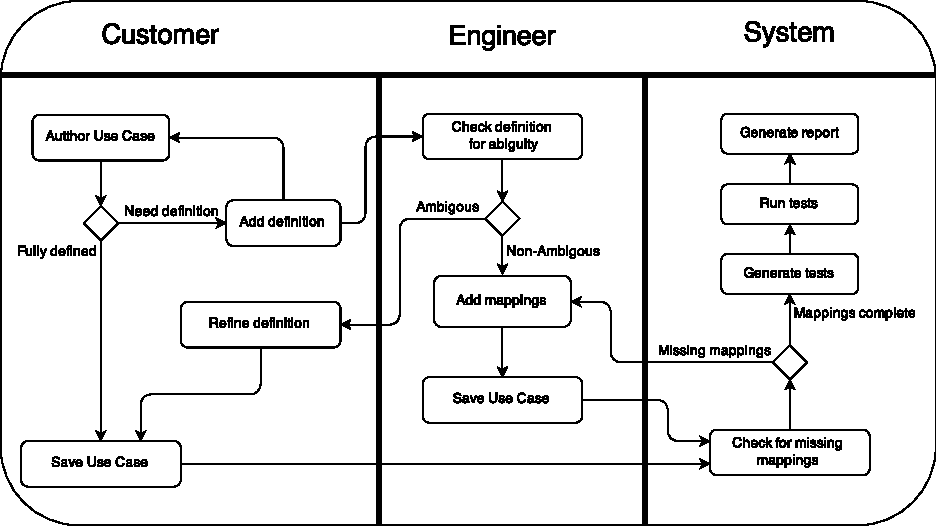
\includegraphics[scale=0.75]{img/use_case_creation_activity_diagram}
\centering
\caption{Use case creation with different actors}
\label{fig:use_case_creation_activity_diagram}
\end{figure}

What is in the customers interest is having acceptance tests match the use cases as closely as possible. Preferably, the should be able to be automated as well. Figure \ref{fig:use_case_creation_activity_diagram} shows an activity diagram involving three actors, the customer, the engineer and the system\footnote{Use case system}. In this diagram, the customer authors use cases while adding missing definitions not already in the tool. A definition is textual description of a concept which may be -- for instance -- an actor, role or action. This description is then given a unique name, that may correspond to a concept already found in the domain model. The domain model, if defined beforehand, could also be thought to be a part of the built-in declarations.

\begin{figure}[h]
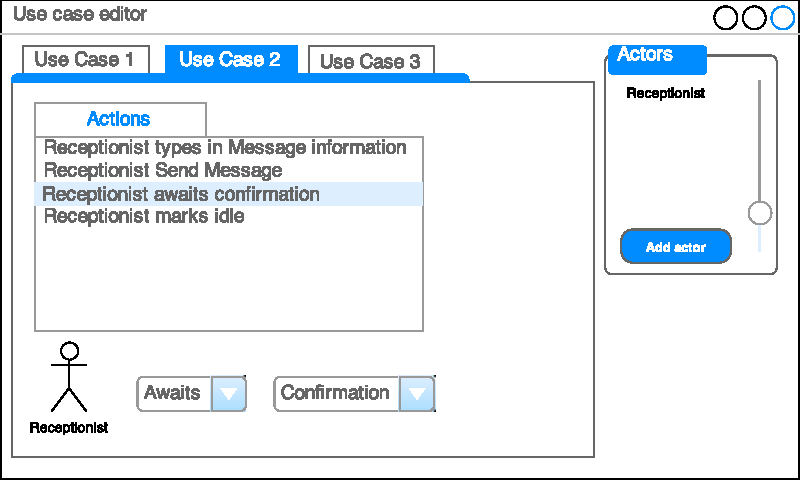
\includegraphics[scale=0.9]{img/test_case_ui}
\centering
\caption{Use case editor UI mockup}
\label{fig:use_case_editor_mockup}
\end{figure}

Whenever there is a new use case, a change to an existing use case, or simply a definition, the system should try to generate tests from the new information. If this step fails it is likely due to insufficient concept mappings. From here, a software engineer must manually map individual definitions to system macro-functionality or, possibly the use case could be linked to an existing manually written test, if the generation step is not possible for some reason. A mockup of a user interface from the customer point of view is shown in figure \ref{fig:use_case_editor_mockup}. A list of available actors (only containing one element, however) is shown on the right hand side. The main part of the window contains the use case currently being worked on. The bottom part of the window is the edit part, where dropdown lists of actions and targets resides.


\section{Proposed solution}
"Side-cart" tool that (maybe) uses natural language processing. The developement is supported by a two-sided approach. Both top-down and bottom-up. Meaning that design an implementation will go hand-in-hand and hopefully lead to a good middle-road.
%TODO something about existing approaches.
%TODO Step-wise go through the enhancement process.
%  - Basically, autogenerate the use case action code line
%  - Infer some Class dependencies, which then becomes Framework dependencies.
%Definition dictionary
% Remember that an actor has a set of goals, which he/she wants to realize through the system. Actor can be  primary (typically people) or supporting (provides service or information) - passive.
% A good goal has a verb/noun combination.
%REMEMBER TO TAKE INTO ACCOUNT <INCLUDE> use cases -- Basically extensions
This section takes starts from a use case description, and tries to go through the steps needed to convert it into an acceptance tests. The use case used in this text is simplified and outlined in verbatim text seen in listing \ref{lst:uc-simple-example}.\todo[inline]{Check context, and make sure it leads in to this.}.
\begin{lstlisting}[frame=single,style=usecase, caption=Use case example, label=lst:uc-simple-example]
Scenario:
  Receptionist types in message
  Receptionist sends message
  Receptionist marks state as ready 
Preconditions:
  The receptionist is created
  The receptionist is logged in
Postconditions:
  The message is stored
  The receptionist is ready to handle the next call
\end{lstlisting} 
Translating this example, we first identify the domain concept contained within the statements in the text. In this case, we here observe that it includes the concept ``message'' a ``receptionist'' actor. additionally; some interaction between the message and the actor, which we define as actions.\\
In listing \ref{lst:uc-simple-example-highlighted} we have highlighted the different parts of the use case, using an orange color for actors, green for actions, blue for domain concepts, and a dark red for attributes. Using this highlight, it illustrates the abstract interpretation and the interaction between the different part very well. It also reveals very clearly which archetype (actor, concept \dots) each of the different parts should have. 
\todo[inline]{More elaborate text here}.
\begin{lstlisting}[frame=single,style=usecase, caption=Use case example with its different parts highlighted, label=lst:uc-simple-example-highlighted]
Scenario:
  @\color{orange} Receptionist@ @\color{dkgreen}{types in}@ @\color{blue}{message}@
  @\color{orange} Receptionist@ @\color{dkgreen}{sends}@ @\color{blue}message@
  @\color{orange} Receptionist@ @\color{dkgreen}{marks state}@ as @\color{blue}{ready}@
Preconditions:
  The @\color{orange}receptionist@ is @\color{dkred}logged in@
Postconditions:
  The @\color{blue}message@ @\color{dkred}is stored@
  The @\color{orange}receptionist@ @\color{dkred}is ready@ to handle the next call
\end{lstlisting} 
Based upon the information in listing \ref{lst:uc-simple-example-highlighted}, we could create an abstract interpretation that generates a test that looks like listing \ref{lst:uc2_example_test_code}.
Each of the concepts in this example is mapped to a class, that could likely be stubbed out automatically by the test tool.\\\\
Given the amount of information in (and markup of) the use cases, we can easily generate code such as the one shown in listing \ref{lst:uc2_example_test_code}. But these functions are still very high-level, and doesn't assert anything about the system being tested. To do this, we need to fill in the methods used on our receptionist and message object.
\begin{lstlisting}[caption=Suggestion of generated test case,label={lst:uc2_example_test_code}]
boolean test (receptionist, message) {
  // Scenario
  receptionist.types_in (message);
  receptionist.sends (message);
  receptionist.marks_state (idle);
  
  // Postcondition
  return
    message.is_stored() AND
    receptionist.is_ready();
}
\end{lstlisting}
Going through the test case, from the top, we can see that the \texttt{receptionist.types\_in~(message)} method operates on the receptionist actor call, and requires knowledge of the ``message'' domain concept. Furthermore, we known from the domain analysis that \emph{is not part} of the use case, that the action of typing in a message is actually a creation of message. So, before being able to test it, we need some way of simulating the message creation and -- more concretely -- fill in the actual message content. Conceptually, this is some sort of content generator. A concrete implementation could be a simply ``dummy object'' or an object that is initialized with random content. Once the message object is mapped to a content generation function, we will be able to fully generate the test. The content generation function would probably still need to be hand coded, as this is example data.\\\\
The next statement; \texttt{receptionist.sends (message)} can be classified as a store function. It takes the argument ``message'' and makes it available for other actors to access later on, by storing it persistently. This is typically done using a database or file store. By mapping a message to a message store, we can remap an ``enqueue'' method of the message object, which needs to have a notion of where it is, or should be stored. This is realized by having a ``messageStore'' interface which is a service interface object that, can actually be originating directly from the code base of the system under test.\\\\
The final statement in the scenario is \texttt{receptionist.returns\_to (ready\_state)}. This is actually a mutation function that alters the state of the receptionist actor. This state change could be global and should then  be updated multiple places, which then leads to additional ``state-store'' dependencies. Here, we also note that there is a concept of a ready\_state this is an explicit state change that could, possibly be linked to a state machine contained within the receptionist actor object.\\\\
The final thing done in the tests, is the postconditions. In this case, we treat the postcondition as a boolean attribute of the concept which it refers to. The general assumption is that pre- and postconditions are expressions that must always be true, and must refer to a concept previously referred to in the scenario. So for the \texttt{receptionist.is\_ready()} predicate we can map it to the internal state of the receptionist being equal to the ``ready'' state.\\\\
The mapping can be described in a textual language such as shown in listing \ref{lst:mapping_language_concept} where we initially state the domain concept name -- which is in this case Receptionist -- and the requirements, properties and mappings it has, plus which functionality it provides. The requirements are which other domain concepts are needed by this one. The properties are the boolean properties that are used in predicates and the ``provides'' section are functions that are either used as internal auxiliary functions, or exported functions that other concepts may use.
%Prior to running the tests, the two objects ``message'' and ``receptionist'' needs to be initialized.
%The question is then how much more needs to be added. Can we use some stereotyping to increase the semantics of the annotated use cases? Such as 'storage' for message, and 'actor' for receptionist.
%So last question; who does what, and how much can be automated?
%The first part of the job; typing in the use cases is a manual process that should be done in close cooperation with -- and preferably by -- the stakeholder involved in the use case. So a use case involving an accountant actor should be typed by a accountant representative expected to be using the system, once finished.

\begin{lstlisting}[caption=example language for mapping concepts,label={lst:mapping_language_concept}]:
Receptionist:
  requires:
    MessageContentGenerator messageContentGenerator
    ReceptionistState currentState = ReceptionistState.Unknown
  
  provides:
    changeState (ReceptionistState rs) -> currentState = rs
  
  maps:
    sends_message (Message msg) -> msg.enqueue()
    types_in (Message msg) -> msg.content = messageContentGenerator.next().content
    returns_to (ReceptionistState newState) -> this.changeState (newState)

  properties:
    is_ready -> receptionistState == ready
\end{lstlisting}
The mappings are, in this conceptual model, alias functions to ``real methods'' already provided in the code base of the software under tests, or to functions of other domain concepts. This is probably not feasible in praxis, and will probably be a programing code template instead.

\begin{lstlisting}[caption=Pseudo code representing Receptionist domain actor,label={lst:code_for_receptionist_domain_actor}]
class Receptionist {
   MessageContentGenerator messageContentGenerator= ...;
   ReceptionistState receptionistState = ...;
  
  void types_in (message) {
  	message.updateContent(messageContentGenerator.content);
  }
  
  void sends (Message message) {
    message.enqueue();
  }
  
  // Alias function.
  void returns_to (State newState) {
  	changeState (newState);
  }
  
  void changeState (State newState){
  	receptionistState = newState;
  }
  
  boolean is_ready() {
    return receptionistState == ready;
  }
}
\end{lstlisting}

\begin{lstlisting}[caption=Pseudo code representing Message domain concept,label={lst:code_for_domain_concept}]
class Message {
  RESTMessageClient messageStore = ...;
  
  void enqueue() {
    messageStore.enqueue(message);
  }

  boolean message.is_stored() {
    messageStore.contains(this);
  }
}
\end{lstlisting}

\begin{figure}
 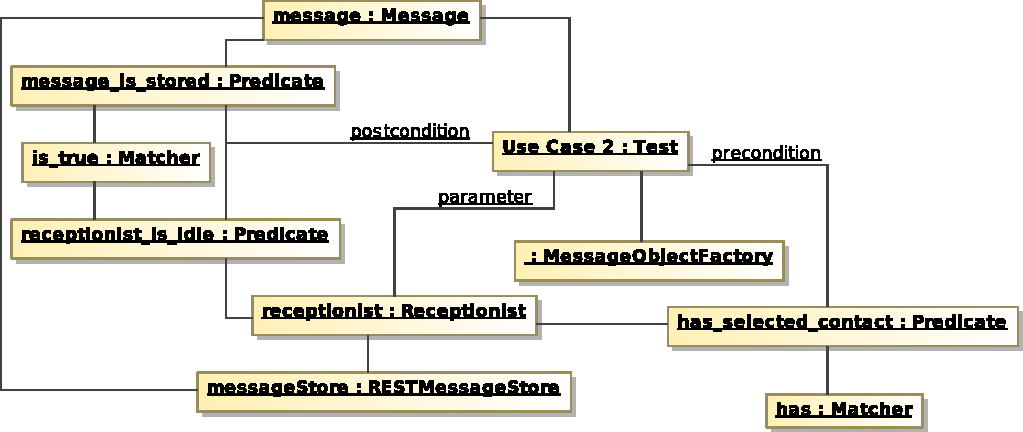
\includegraphics[scale=0.45]{img/uc2_test_config}
 \caption{Object diagram showing the use case as mapped test}
\end{figure}
The function mappings are done in the current solution, by manually writing up the logic needed in a support library, that in many situations reuse the framework directly. For instance, for every service, we have made a client class that, similar to RMI or WSDL handles all the low-level serialization and deserialization work. 

This enables us, in our tests to merely require that an interface (a client of it, that is) is provided to use, rather than having to explicitly elaborate the code in the test case.

%TODO Brief discussion on randomizers.

\begin{figure}
 \centering
 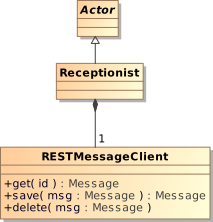
\includegraphics[scale=0.60]{img/support-tools-recepionist-example}
 \caption{support-tools-recepionist-example}
 \label{fig:support-tools-recepionist-example}
\end{figure}

%\begin{figure}
% \centering
%\missingfigure[figwidth=6cm]{This is some text that is with the todo and in the figure}
% \caption{support-tools-recepionist-example}
% \label{fig:support-tools-recepionist-example}
%\end{figure}
\chapter{Case project}
This project uses the open source project ``OpenReception'' as case study. The project aims to provide a drop-in replacement for an existing system, and therefore has relatively fixed requirements that are extracted from the workings of the existing system. The system is developed and released under an open source license and any implementation details are therefore public domain and not covered by any non-disclosure agreements. This section gives a short introduction to the system, its architecture and design and the development process that ultimately motivated the test approach, that is the topic of this thesis.\\\\
OpenReception web-based software/telephony system. It is a system designed to enable receptionists to handle incoming calls, and provide then with the appropriate information so that they may divert or directly handle the calls. The system is designed with high availability in mind with many -- largely independent -- components that are loosely coupled. This limits the Domino-effect, where one faulty component can take down another for no other reason than the fact that they are partitioned together.\\ This component-oriented design has also helped the testing process, as it enabled individual components to be tested and verified independently of the others.

\section{Project scope}
The fundemental requirements for the system originates directly from the fact, that is is supposed to be a drop-in replacement of an exisiting system. It should therefore, as a bare minimum, mirror the features of the existing system.\\
However, the current system has been in production for over ten years and lessons-learned has taught the customer how the system should be improved. %TODO maybe add a list of requirements.

%Use cases are stored in a wiki.


\begin{figure}
  \centering
 
  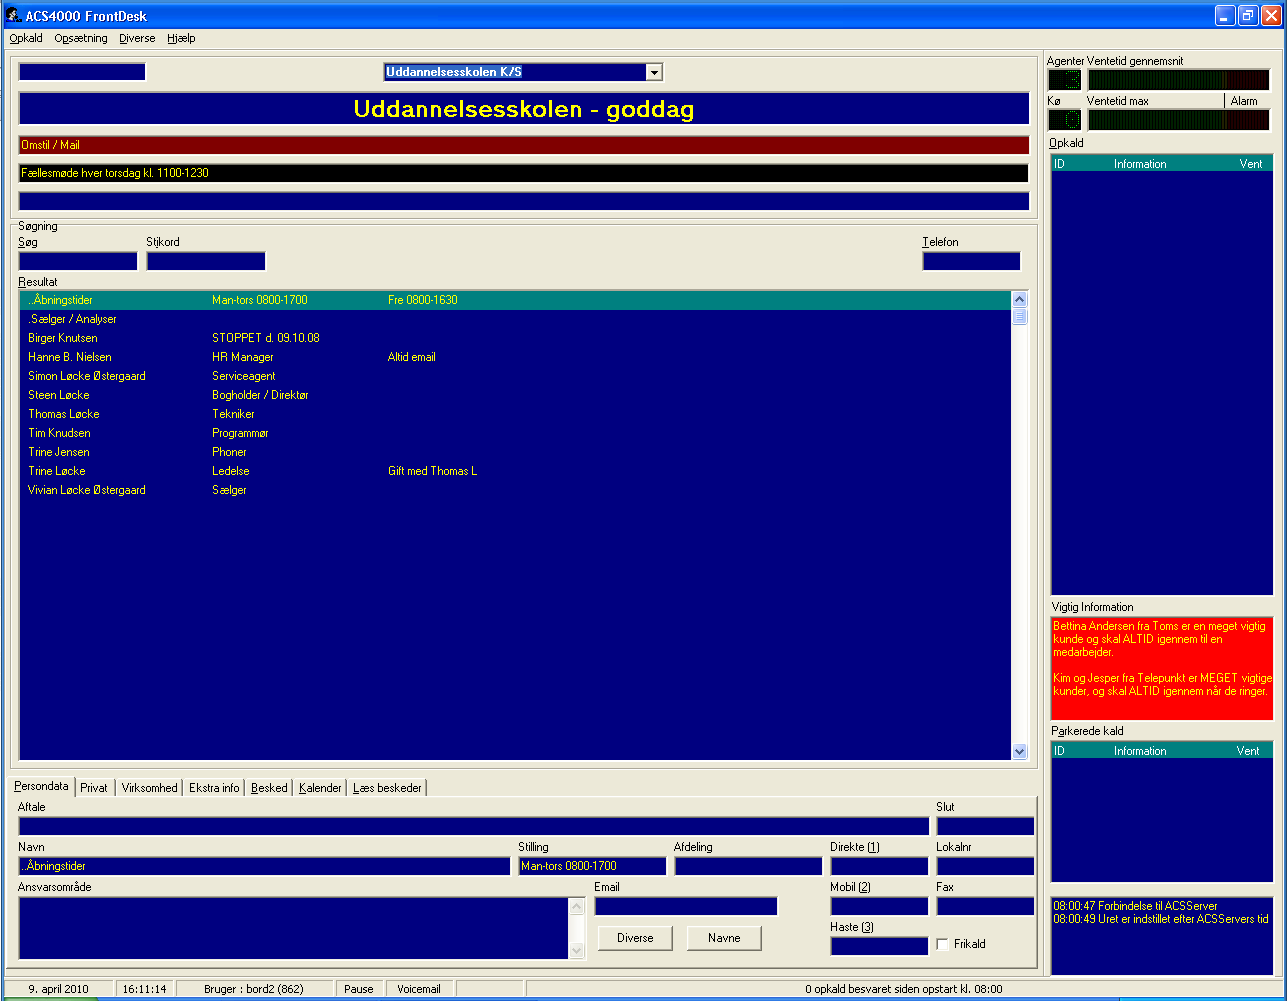
\includegraphics[scale=0.2]{img/frontdesk-client-ui.png}
  \caption{Receptionist client user interface of existing system}
  \label{fig:frontdesk-client-ui}
\end{figure}

\begin{figure}
  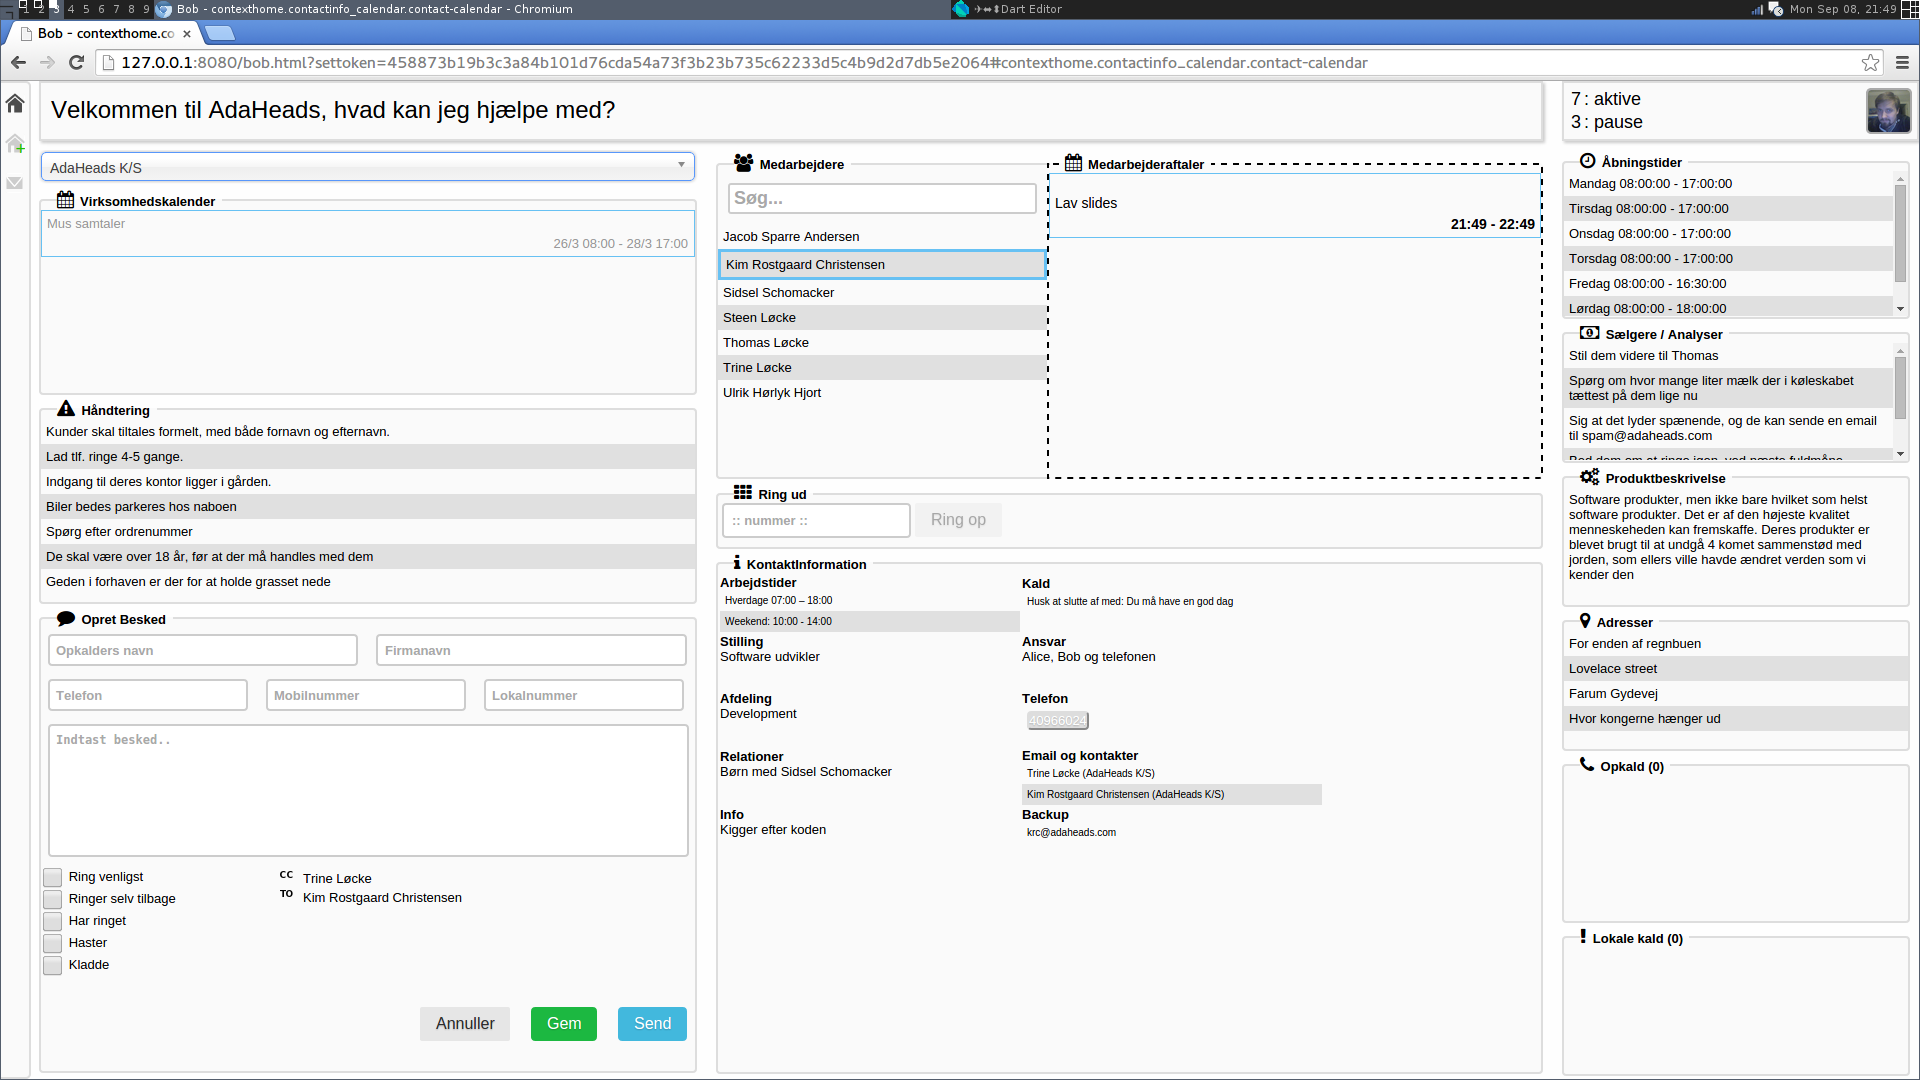
\includegraphics[scale=0.2]{img/openreception-client-ui.png}
  \caption{Receptionist client user interface of OpenReception system}
  \label{fig:openreception-client-ui}
\end{figure}

\begin{figure}[h]
%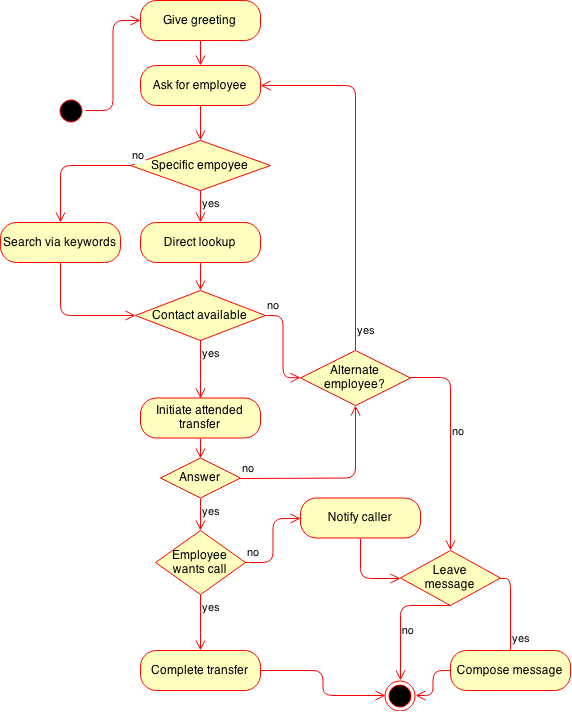
\includegraphics[scale=0.4]{img/activity_diagram_receptionist}
\centering
\caption{Activity diagram for the receptionist actor}
\label{fig:activity_diagram_receptionist}
\end{figure}


%\section{Related work}
%\subsection{Writing requirements as tests}
%\subsection{Writing requirements in formal language}

\section{Brainstorming}
The problem in attaining broad coverage of use cases, and therefore completeness in requirements i primarily that, from the customer perspective, that they feel very overly-verbose and usually too formal in nature. For software engineers, the opposite is usually the case. They feel that the use case descriptions are not structured nor elaborate enough for use in, for instance, code stub generation.

More structure, however, could be helped along the way with proper tooling. Hiding some of the complexity of the constrains of a data model behind a simple user interface supplying dragable components and providing immediate visual feedback in the form of textual use case representation (or a diagram) could "cheat" the customer into adding the needed structure to the use case model.

\begin{figure}[h]
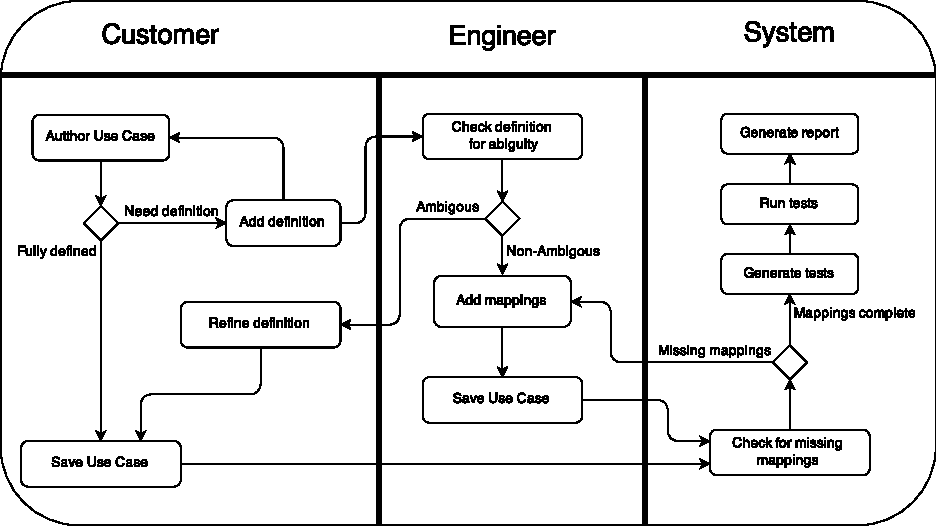
\includegraphics[scale=0.9]{img/use_case_creation_activity_diagram}
\centering
\caption{Use case creation with different actors}
\label{fig:use_case_creation_activity_diagram}
\end{figure}

What is in the customers interest is having acceptance tests match the use cases as closely as possible. Preferably, the should be able to be automated as well. Figure \ref{fig:use_case_creation_activity_diagram} shows an activity diagram involving three actors, the customer, the engineer and the system\footnote{Use case system}. In this diagram, the customer authors use cases while adding missing definitions not already in the tool. A definition is textual description of a concept which may be -- for instance -- an actor, role or action. This description is then given a unique name, that may correspond to a concept already found in the domain model. The domain model, if defined beforehand, could also be thought to be a part of the built-in declarations.

\begin{figure}[h]
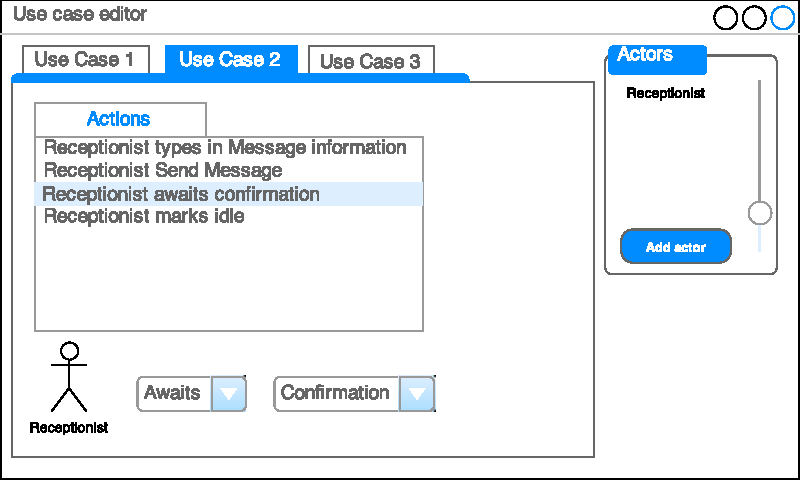
\includegraphics[scale=0.9]{img/test_case_ui}
\centering
\caption{Use case editor UI mockup}
\label{fig:use_case_editor_mockup}
\end{figure}

Whenever there is a new use case, a change to an existing use case, or simply a definition, the system should try to generate tests from the new information. If this step fails it is likely due to insufficient concept mappings. From here, a software engineer must manually map individual definitions to system macro-functionality or, possibly the use case could be linked to an existing manually written test, if the generation step is not possible for some reason. A mockup of a user interface is shown in figure \ref{fig:use_case_editor_mockup}.

% Something about generating partially-automated tests, where the system sets up everything for the customer and then notifies them about the next steps they have to take to move the test forward.

\section{Extracting semantic}
Example; in the use case it is stated that a call is hung up and a callee awaits this event. The lifeline of the call is however not tracked and to be able to properly assert the true state of this, the code macro needs to into account this lifeline and reflect on which assertions hold for every stakeholder that has knowledge of the call. % TODO: Elaborate the example and explain that a phone call is a good example because it has an A and B-leg and potentially a system that tracks its state.

\subsection{Letting the customer inject semantics}

There are two basic approaches to letting the customer inject semantics into the requirements. The first is to do a full up-front declaration of every term used within the problem domain and supply this as a toolbox for the customer %todo example.
The other approach is to do it on the go by outlining concepts as stubs whenever they appear. This approach is similar to what is used in wiki software. %todo eaxmple

\section{Class-responsiblity-collaboration cards}
%Nouns should turn into the classes of the card, verbs typically turn into the responsibilities of the card, and collaborators are the other cards with which the card will be interacting with.
%FROM: http://en.wikipedia.org/wiki/Class-responsibility-collaboration_card

\section{Verification problem}
A big issue in software

\section{End-user experience}
%The challenge in documenting requirements is, and has always been, to formulate them on a non-ambiguous form. The quantification of ambiguity tends to be difficult as well, due to the fact that requirements are usually formulated in natural languages following some rules, such as pre-defined glossary and constraints. Constraints vocabulary typically consists of should, could, may, must.

%As requirements are basically constraints to your system, a subset of them may be expressed as expressions following a formality that is machine-interpretable. Vienna Development Method (VDM) and Z notation are two approaches that tries to formally describe systems on a very high level, so that model-checking can be performed on it prior to programming.

An example UI is Starting from scratch, the user would be expected to initially define at least one actor and add a sequence of actions that the actor perform.

%Other method
Wiki-collaboration to "lazily" define the problem domain and verification conditions along the way.

\section{Test setup}
%scaffolding and harness

\section{Formulating requirements}

\section{Framework discussion}
\subsection{Metrics}
% How many lines of code is the support tools? The middleware framework?
% How is it compared to the activity count in the activity diagram?
\subsection{Recommended test framework guidelines}
%Use allocation pools
%Use interfaces a objects.

\section{Requirements as communication platform}

Avoid technical jargon (\cite{christel1992issues})

\section{Related work}
\subsection{FIT Framework}

We've taken an offset in use cases, but there could be other ways of structuring the requirements of a system, such as the SCRUM user story format;
%Use the SCRUM approach. Don't describe a feature as
%"It should be doing this and that in the following way"
%While the sentence above describes all you need to know to implement the feature, it does not justify the feature. My SCRUM book says features should be written down as a story. A story looks like this:
%"As a <user-role>
%I need a <functionality>
%So that I get <business value>"
%A feature that cannot be justified using such a story is an unjustified feature and thus there is no use to actually implement it.
%E.g.
%"As a visitor of a web portal I need a way to authenticate, so I can access my customer data, but nobody else can"
%Now you don't only know that you need an authentication for your web portal, you also know who needs it (the visitors, basically everyone planing on using it more intensively) and you also know why it is needed, as it gives the user some value.
%Other examples:
%"As a passenger I need a list of all my booked journeys, so that I know when I'm going to travel where and won't lose the overview"
%"As a book keeper, I'd like to have the sales tax being automatically printed to each bill based on customer data, so that I don't have to enter it manually each time I'm printing a bill"
%If every feature needs to be written like that, you'll automatically see if a feature is for the customer, because it is really necessary, or just something your boss/company wants to have and also why they want to have it (what is the big picture behind it? Why are they doing it?).


\section{Use case writing level}
Should not be used to describe UI actions% http://alistair.cockburn.us/Use+cases%2c+ten+years+later (Use case limits).

Use cases expresses expected system behavior. Keep use cases free of UI-action.

There are several levels on which use cases can be written as per\cite{cockburn??}. In our case, it would make the most sense to use the "system" level, as business level is something that is nearly useless because it is largely out of scope. The business logic is also, more elaborately (and implicitly) formulated within a system-level use case. In the other end, a component use case is also very impractical, as our target audience would be people that does not know anything about the specifics of the system being built.

%Note;
An important aspect to keep in mind is that context is important. Writing hundreds of pages of detailed requirements are bound to be decoupled and lose context, and coherence with each other. Deciding on a level that keeps context is important.

\section{Expressing requirements}
%Requirement gathering and documentation often feels a lot like stating the obvious, and being overly-verbose.

\section{Use case translation}
%TODO Add a section on multiple actors and race conditions. How do you create a use case that contains multiple simultanious instances of actors that perform the same action synchronously? Basically asserting parallel properties.

This section tries to extracts an abstract interpretation of a use case through a brief study of two use cases. The goal is to come up with a meta-model of use cases that captures the essentials of the informally written use case, and allow us to map the concepts from it to an abstract syntax so that test code may be generated from it.
\section{Use case semantics}
In order to help the computer make more sense of our use cases, we need to define to it what a use case is. But since a use case is neither strictly defined nor standardized anywhere, we need to pick a suitable representation.
To help us extract some machine-understandable structure -- or merely semantics -- of use cases, we've hand-picked two use cases from our case study system.\\\\
The first use case is a basic phone call forwarding session that goes though a receptionist. The use case is described from the receptionist's point of view, as this is the scope of the main case study system. The use case has a detailed description in schema form in figure \ref{fig:uc1}. \\\\
The second use case is, in a sense, embedded in the first one as it part of the extensions of that use case. This will be covered later on. The use case covers a ``send message'' session typically done by having the receptionist actor transcribe a spoken message along with caller information (name, company, ...) onto a set of text input fields that then can be assembled to a message. This message is then handed over to the system that may enqueued it for later delivery -- or send it immediately, depending on implementation.

\subsection{Identifying concepts}
The first concept we know, for certain, should got into our meta model is the use case. It serves as our top-level concept that every other concept, in some way, relates to. From here on, we go back to our two case study use cases use cases where we can easily -- by manual inspection -- identify various concepts that most likely also belongs in a domain model. In use case 1 (figure \ref{fig:uc1}), we see three different actors: A receptionist, a contact and a caller. We also have a primary actor that provides us with the ``glasses'' we see the use case through. This, in conclusion, means that we need an actor as part of our domain model, and an association between a use case and an actor.\\\\
Skipping the pre- and postconditions for now, we take a look at the ``Main success scenario'' and see that, broadly speaking, each use case action involves one actor performing an action, possibly affecting a target object -- which could be another actor. For the purpose of generating tests, it is not important that actors may target other actors though their actions, and this association is therefore left out of the meta model.\\\\
Given the loose structure of the use case concept, we believe it is sufficient to treat preconditions as simply other use cases. A more elaborate motivation for this can be found in section \ref{sec:test_case_state}.\\\\
Postconditions are defined to be predicates. This is because they share the common trait that they must be true, for the given expression to be true. In our case, the postcondition ``Receptionist is ready for next call'' states the actor receptionist that is participating in this use case, must be in a specific state when the last statement of the use case is done. A postcondition should refer to an actor, target or action previously defined in the use case to avoid redundant mapping. The predicate itself can be some sort of quantifiable strict logic such as ``Message has recipients'', or could as an extension be defined as the more loose ``Message should have recipients'', which should map to a warning in the generated tests, rather than an error.

Pre and post-conditions are operations that work on expressions rather than statements

Alternate scenarios are not yet covered.

\subsection{Meta model}
This section contains a brief discussion of a meta model that could be used for translating use cases into test cases. The discussion is supported by the graphical model depicted in figure \ref{fig:meta_model}\\\\
Within the definition mapping, the mapping class denotes the relation between either a predicate and a predicate expression, or a statement (indirectly by the actor, action, target composition). The mapping is uniquely defined by mapping by its composition of an actor, an action and a target, as it should be safe to assume that ``The contact accepts the call'' means the same no matter which use case it appears in. Each mapping will imply a requirement on a resource, which can be any actor or target. The are basically constraints stating the minimum functionality the test framework\footnote{Domain-specific scaffolding code that needs to be written by hand} should have to make the generated test code runnable. These resources could, in test code frameworks, be provided by factory classes or object pools.\\\\
Tests are the output of a sequence of mappings, that has a state which is then defined by the mappings that originally defined the test. The test will also have references to the predicate expressions that are outputted by mappings as well.

\begin{figure}[h]
  \centering
 
  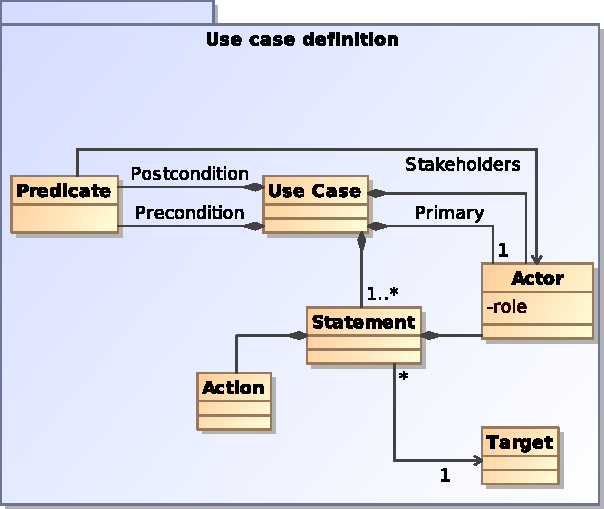
\includegraphics[scale=0.72]{img/use_case_meta_model}
  \caption{Intermediate meta model for use case representation along with tests}
  \label{fig:use_case_meta_model}
\end{figure}

\begin{figure}[h]
  \centering
 
  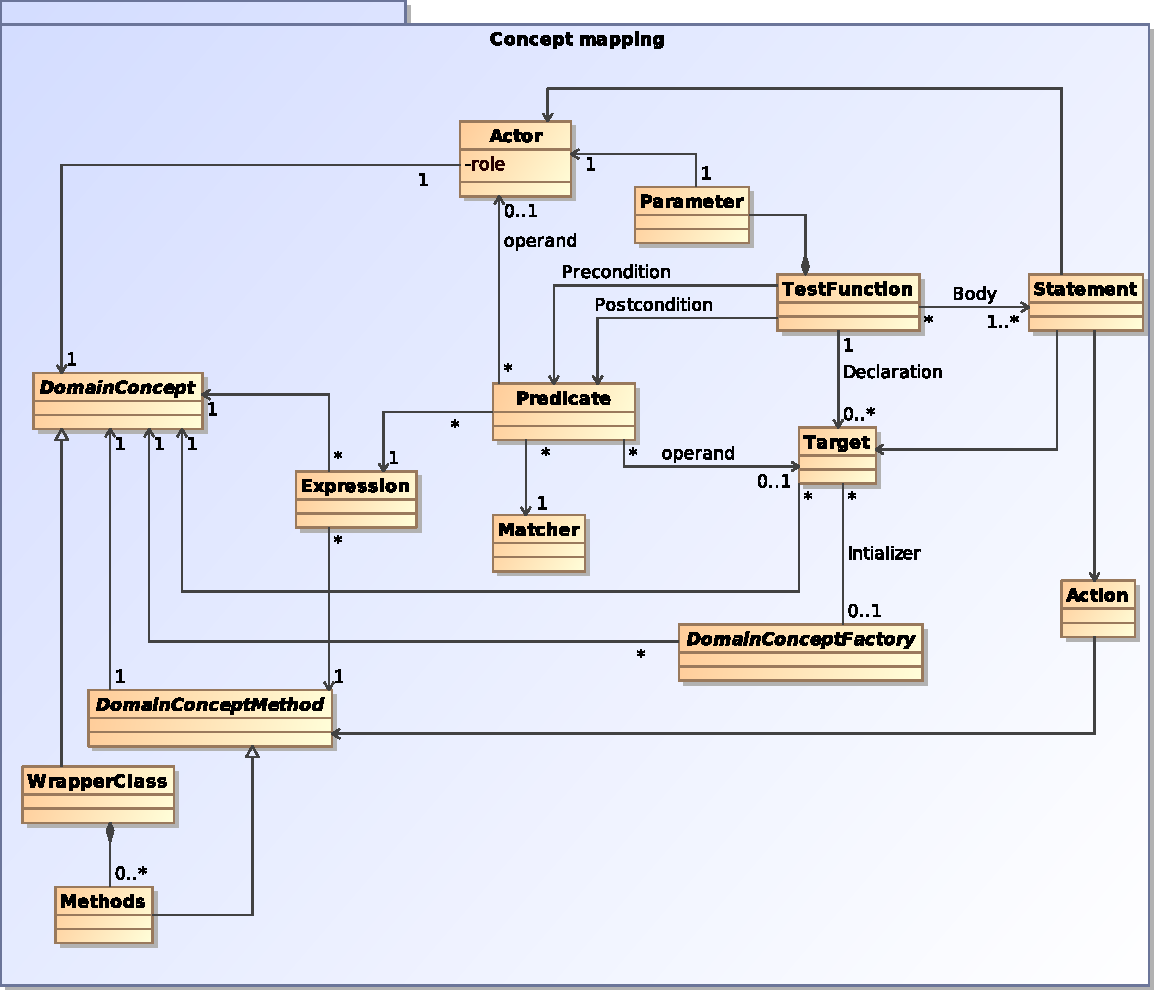
\includegraphics[scale=0.72]{img/use_case_mapping}
  \caption{Use case mapping}
  \label{fig:use_case_mapping}
\end{figure}

\section{Mapping manually}
Within a use case there are some bits of implicit knowledge that we need to extract. To begin with, we observe that for the use cases in figure \ref{fig:uc1} and \ref{fig:uc2}, there are domain actors involved.

Each involved domain actor will then be mapped to a wrapper class that represents the domain object, and could possibly extend a class from the implemented code base.

In order to get the actor object to perform actions, we need to map the actions in the use case to some functions associated with the actor class. These functions could be a direct link to a method that is part of the main codebase which is tested against, a new method written specifically for this purpose - or a macro function that combines functionality from different domain concepts in a single functions.

Whenever there is a mention of an object (a target of an action) which could be, for instance, a message object we assume that its the same object that is tracked during the entire use case. So, from use case 2, we have ``Receptionist sends the message via the system'' in the main success scenario and ``Message is stored and ready for dispatching'' in the postconditions.

Regarding the test as a function

%\section{Object tracking} NOTE: Maybe something about object lifecycles (and statemachines for them) here.

\section{Test case state}
A test consists of three basic steps; setup, run and teardown. Setup and teardown is different from pre- and postcondition in that they are unrelated to the test itself, they merely make sure that objects are initialized with right values and, in general, are in the state that the test expects.

There needs to be an executable domain model programmed, not necessarily complete, but the concepts covered in the use cases should at least be there. So for \ref{fig:uc2}. We need at least a class representing the actor ``Receptionist'', and a class representing a message. The actions performed by the actor could then either be class methods, or simply functions taking the primary actor (or more exact; classes of the actor), as an argument.


%NOTE: The test mapper will then select the "essentials" of the sentence, which could be just the verb, noun and object.
\label{sec:test_case_state}


\section{Test case example}
\begin{lstlisting}
void use_case_1 (Receptionist receptionist) {

   MessageObjectFactory messageObjectFactory = new MessageObjectFactory();
   Message message = messageObjectFactory.create();

   // Preconditions
   Matcher.has (selected_contact (receptionist));

   // Use case body 
   receptionist.types_in(message);
   receptionist.sends(message);
   receptionist.marks_state_idle();

   // Postconditions 
   Matcher.is_true (is_stored (message));
   Matcher.is_true (is_idle (receptionist));
}
\end{lstlisting}

\begin{figure}
  \centering
 
  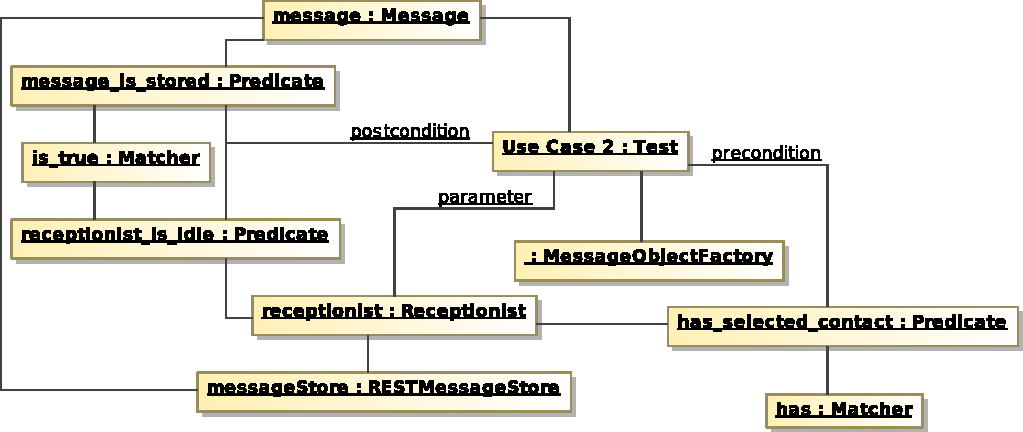
\includegraphics[scale=0.6]{img/uc2_test_config}
  \caption{object diagram depicting the configuration of use case 2}
  \label{fig:uc2_object_diagram}
\end{figure}


\begin{figure}[h]
  \centering
\begin{usecase}

\addtitle{Use Case 1}{Transfer to contact} 

%Scope: the system under design
\addfield{Scope:}{System-wide}

%Description: A brief description of the use case
\addfield{Description:}{The receptionist actor must be able to transfer an active call to a chosen -- dialed -- contact associated with the currently active reception}

%Level: "user-goal" or "subfunction"
\addfield{Level:}{User-goal}

%Primary Actor: Calls on the system to deliver its services.
\addfield{Primary Actor:}{Receptionist actor}

%Stakeholders and Interests: Who cares about this use case and what do they want?
\additemizedfield{Stakeholders and Interests:}{
	\item Receptionist: Wants to process the call with regards to the caller's wishes
	\item Caller: Wants to reach a specific contact
}

%Preconditions: What must be true on start and worth telling the reader?
\additemizedfield{Preconditions:}{
      \item Receptionist has picked up incoming call from caller
      \item Receptionist has parked incoming call
}
%when multiple
%\additemizedfield{Preconditions:}{} 

%Postconditions: What must be true on successful completion and worth telling the reader
\additemizedfield{Postconditions:}{
      \item Caller and contact's phones are connected
      \item Receptionist is no longer in call and ready for next call      
}
%when multiple
%\additemizedfield{Preconditions:}{}

%Main Success Scenario: A typical, unconditional happy path scenario of success.
\addscenario{Main Success Scenario:}{
      \item Receptionist dials a number of the selected contact
      \item The contact accepts the call (picks up)
      \item Receptionist has a dialogue with contact
      \item Receptionist transfers contact to caller
      \item Receptionist marks his/her state as idle.
}

%Extensions: Alternate scenarios of success or failure.
\addscenario{Extensions:}{
	\item[2.a] Contact cannot be reached
		\begin{enumerate}
		\item[1.] Receptionist tries alternate contact
		\item[2.] Receptionist returns to step 1
		\end{enumerate}
	\item[3.a] Contact declines transfer
		\begin{enumerate}
		\item[1.] Receptionist hangs up contact
		\item[2.] Receptionist picks up caller
		\item[3.] Receptionist offers caller to leave a message
		\item[4a.] Caller wishes to leave a message
		\begin{enumerate}
			\item[1.] Receptionist types in message and caller information
			\item[2.] Receptionist saves message
		\end{enumerate}
		\item[4b.] Caller does not wish to leave a message
		\item[5] Receptionist ends call with caller
		\item[6] Receptionist returns to step 6
		\end{enumerate}
}

%Special Requirements: Related non-functional requirements.
%\additemizedfield{Special Requirements:}{
%	\item first applicable non-functional requirement
%	\item second applicable non-functional requirement
%}

%Technology and Data Variations List: Varying I/O methods and data formats.
%\addscenario{Technology and Data Variations List:}{
%	\item[1a.] Alternative first action with other technology
%}

%Frequency of Occurrence: Influences investigation, testing and timing of implementation.
%\addfield{Frequency of Occurrence:}{}

%Miscellaneous: Such as open issues/questions
%\addfield{Open Issues:}{}

\end{usecase}
   \caption{Use case 1: Forward call to contact}
  \label{fig:uc1}

\end{figure}

\begin{figure}[h]
  \centering
\begin{usecase}

\addtitle{Use Case 2}{Send Message to contact} 

%Scope: the system under design
\addfield{Scope:}{System-wide}

%Description: A brief description of the use case
\addfield{Description:}{A receptionist must be able to send a message -- via a distribution list -- to a contact, typically containing information received verbally via a call. An example use case, from the receptionist actor point of view is outlined below.}

%Level: "user-goal" or "subfunction"
\addfield{Level:}{User-goal}

%Primary Actor: Calls on the system to deliver its services.
\addfield{Primary Actor:}{Receptionist actor}

%Stakeholders and Interests: Who cares about this use case and what do they want?
%\additemizedfield{Stakeholders and Interests:}{
%	\item Receptionist: Wants to process the call with regards to the caller's wishes
%	\item Stakeholder 2 name: his interests
%}

\additemizedfield{Preconditions:}{
      \item Receptionist have selected a contact who will serve as message recipient
} 

%Postconditions: What must be true on successful completion and worth telling the reader
\additemizedfield{Postconditions:}{
      \item Message is stored and ready for dispatching
      \item Receptionist is idle
}

%Main Success Scenario: A typical, unconditional happy path scenario of success.
\addscenario{Main Success Scenario:}{
      \item Receptionist types in message
      \item Receptionist sends the message via the system
      \item Receptionist marks his/her state as idle.
}

%Extensions: Alternate scenarios of success or failure.
%\addscenario{Extensions:}{}

\end{usecase}
   \caption{Use case 2: Send message to contact}
  \label{fig:uc2}
\end{figure}

%TODO Integrate and finalize notes below.

%\section{Test framework}
% You need to write a test framework containing object pools, factory classes aso.
%\subsection{Exploiting injected semantics}
%How may we benefit from additional semantics? We can identify rubbish postconditions, such as predicates that involve objects that are either not modified in the statements, or simply never referenced.

%\section{Evaluating a use case}
%A use case can be modeled as a function taking in a starting environment and returning a boolean value, so $U \rightarrow env \rightarrow bool$

%The expression of a use case that consists of $n$ statements then becomes: 
%$Postcondition \rightarrow S_n \rightarrow S_{n-1} \rightarrow \dotsb \rightarrow S_2 \rightarrow S_1 \rightarrow Precondition \rightarrow env$
%The expression function is applied to the statement, then the result is applied to the matcher which then returns a success or failure value depending on the outcome of the evaluation.
%\texttt{matcher expression} ($s$)

%Test case; when does it end? in our case, the message-sending archtecture is defined to be a work-queue where the dispatcher is decoupled from the message sending, which is merely an enqueuer. If the postcondition for our test case had been; "Message is received by contact", then the test-macro function becomes increasingly large.
%Test cases may further introduce dependencies, such as messageStore


\section{Targeted requirements}
We've chosen to focus on the requirements that involves core features from the Receptionist actor point of view. These are, on a high level;
\begin{description}
  \item[Manage calls:] Being able to technically handle calls by performing receive, park, transfer and hangup action.
  \item[Process calls:] Being able to process calls in the context of a dialed reception. This involves having access to data about the reception and its contacts. Being able to dial them, or send them a message.
  \item[Manage message:] Being able to send out messages to contacts, view and resend existing messages.
\end{description}

For our targeted use cases, we've cherry-picked some specific paths from the activity diagram for the receptionist actor (see figure \ref{fig:activity_diagram_receptionist}).

\begin{description}
  \item[UC1: Transfer to contact:] A receptionist must be able to transfer a call to a chosen contact associated with the currently active reception. An example use case, from the receptionist actor point of view is outlined below.
  \begin{itemize}
    \item Preconditions.
    \begin{itemize}
      \item Receptionist is handling picked up incoming call $A$
      \item Receptionist has parked call $A$
    \end{itemize}
    \item Actions.
    \begin{itemize}
      \item Receptionist dials the number of the selected contact (call $B$)
      \item Receptionist hears dial tone
      \item The contact's phone is ringing.
      \item The contact accepts the calls (picks up)
      \item Receptionist has a dialogue with contact
      \item Receptionist transfers call $B$ to call $A$
      \item The system breaks the receptionist's connection to both call $A$ and $B$    
      \item Receptionist marks his/her state as idle.
    \end{itemize}
  \end{itemize}

  \item[UC2: Send message to contact:] A receptionist must be able to send a message -- via a distribution list -- to a contact, typically containing information received verbally via a call. An example use case, from the receptionist actor point of view is outlined below.
  \begin{itemize}
    \item Preconditions.
    \begin{itemize}
      \item Receptionist may have previously received a call $A$, which may still be active.
    \end{itemize}
    \item Actions.
    \begin{itemize}
      \item Receptionist finds contact $C$ who will serve as recipient
      \item Receptionist selects $C$
      \item Receptionist types in message
      \item Receptionist sends the message via the system
      \item Receptionist marks his/her state as idle.
    \end{itemize}
  \end{itemize}
\end{description}

%TODO High leve description (customer level)

\chapter{Validating implementation}
%Something about the V-model.

\section{Formalized approaches}
%2.1. Use case description
%A semiformal use case description is simply a natural
%language text structured using a text template which divides
%the text into logical parts. Even though there is no broadly
%accepted standard use case template, the existing templates
%are quite similar.
\section{Testing}
%Fixtures
%Design by contract
%Harness

\section{Regression testing}

\chapter{Requirement formalization}
Actors, Roles

Aspects. Behavior. State space.

\section{Use case as base}
%\includegraphics[scale=0.4]{img/req_meta.png}

\subsection{What to include?}
From \cite{Cockburn:2000:WEU:517669} we get;
\begin{quote}
``... The use case, as the contract for behavior, captures \emph{all and only} the behaviors related to satisfy the stakeholders’ interests.''
\end{quote}

\section{Processes}

\chapter{Test generation}
Using -- exclusively -- the use case from \textbf{RQ2} as base, we try to derive what is needed in order to generate a basic test.
To achieve the minimum implementation, we cut away the optional precondition that may be covered by other use cases. After this, we see an implicitly \emph{ordered list of actions} that we need to succeed in order for the test to be a success. There is an actor that performs an action at each step. The system, in its entirety, may also be referred to as an actor as it is also capable of performing actions.

So, summing up, we have;
\begin{itemize}
  \item This use case consists of an ordered list of actions, where actions consist of
  \begin{itemize}
	\item One or more actors
	\item One verb describing the action
	\item One target for the action (object for verb)
  \end{itemize}
\end{itemize}
If we 

\section{Requirement/test mapping}
%The communication model needs to be known.

We consider a use case to a flow events that mutates a state...


\section{Environment}
Traversing the use case is considered a long function call-chain. Each new procedure call passes along the current global state onto the next procedure. This method of passing along the state is a common pattern is interpreters and compilers, where the global state is referred to as "the environment". In our test-case compiler we adopt this approach. One of the large benefits is to have the ability to have an exit procedure that performs state clean upon exit of every use case. These procedures should run regardless of exceptions raised within the call-chain, but respond to them. This behavior is identical to the functionality seen in "teardown" functions in test framework for programming languages. See section \ref{sec:test_framework_programming} for a discussion on these frameworks.\\\\
The environment should contain the current state within the scope of test currently running. By state is meant any objects created or modified during the test.

\chapter{Process evaluation}

%\section{Applicablity to different methodologies} See http://en.wikipedia.org/wiki/Requirements_analysis
% Waterfall, Prototype model, Incremental, Iterative, V-Model, Spiral, Scrum, Cleanroom, RAD ...


% Further work
%  - Misuse case
%  - Validating event chain against a state machine (automaton).
\chapter{Conclusion}

\bibliographystyle{plain}
\bibliography{references}

\nocite{*}

\end{document}
